\documentclass[a4paper,10pt]{memoir}
\usepackage[italian]{babel}
\usepackage{wrapfig}
\usepackage[pdftex]{graphicx}
\usepackage{graphviz}
\usepackage{amsmath}

\usepackage[chapter]{minted}
\usepackage{adjustbox}
\usepackage{hyperref}
\hypersetup{
  colorlinks   = true,    % Colours links instead of ugly boxes
  urlcolor     = black,    % Colour for external hyperlinks
  linkcolor    = black,    % Colour of internal links
  citecolor    = black      % Colour of citations
}

% import package
\usepackage{FrontespizioSapienza}

% declare info
\FSSTitolo{Ottimizzazione delle risorse nell'uso di servizi in background in SeismoCloud per Android}
\FSSFacolta{Facoltà di Ingegneria dell'Informazione, Informatica e Statistica}
\FSSCorso{Informatica}

\FSSCandidato{Enrico Bassetti}
\FSSMatricola{1401568}
\FSSRelatore{Emanuele Panizzi}
\FSSCorrelatore{}
\FSSAnnoAccademico{2016/2017}


\begin{document}
  
  
\frontmatter


% print title
\maketitle
\cleardoublepage

%\vspace*{10cm}
%\begin{flushright}
%\textsl{...}
%\end{flushright}
%\cleardoublepage

% rest of the document
\begin{abstract}
	\thispagestyle{plain}
	L'oggetto della tesi è lo studio (e l'applicazione) di modifiche al codice dell'applicazione per Android chiamata \textbf{SeismoCloud}, modifiche che hanno lo scopo di migliorare il funzionamento e ridurre lo spreco di risorse. In un momento in cui gli \textit{smartphones}, pur essendo carichi di processori potenti e più capacità, fanno fatica a contenere ogni \textit{app} che l'utilizzatore installa ed arrivare a fine giornata \textit{carichi}, \textbf{è di vitale importanza utilizzare al meglio le risorse a bordo del telefono}: la batteria in primis, ma anche il tempo di CPU, la memoria occupata e la connessione alla rete Internet.
	
	\medskip
	
	L'applicazione \textit{SeismoCloud} è mediamente più ``vorace" di risorse rispetto alla media delle altre applicazioni; il motivo è il suo scopo: è parte fondamentale di un sistema di rilevamento terremoti, in inglese \textit{Earthquake Early Warning system}, capace di individuare i terremoti nell'istante in cui emergono in superficie, e di avvertire le popolazioni vicine. Per far questo, la \textit{app} è dotata \textbf{di un servizio attivo in background}, che ha lo scopo di individuare le scosse di terremoto presenti dove il telefono è posizionato.
	
	\medskip
	
	Fare una analisi accurata delle risorse necessarie, in fase di progettazione di sistemi come questi, non è facile: la velocità con cui gli \textit{smartphones} acquistano funzionalità e cambiano il modello di utilizzo è elevata, ed inoltre alcune implementazioni algoritmiche possono dare risultati inaspettati, vista la grande differenza tra un dispositivo ed un altro. Ecco quindi che una fase di studio parallela allo sviluppo è stata d'aiuto per rendere più efficiente il codice scritto (anche grazie ai test effettuati su un numero di dispositivi differenti).
	
	\medskip
	
	La tesi è divisa in 4 parti fondamentali: lo studio sull'\textbf{ottimizzazione energetica}, ovvero come evitare di consumare batteria pur mantenendo attive le funzionalità utili; lo studio sull'\textbf{ottimizzazione dell'uso della rete Internet}, visto che ha impatto sia sulle reti dati ``a consumo", sia sulla stessa batteria (per il consumo delle antenne); dopodiché sono presenti ottimizzazioni algoritmiche che hanno \textbf{diminuito il carico sulla CPU e sulla memoria} del telefono; ed infine abbiamo \textbf{integrato un processo di sviluppo che permette di monitorare (ed evitare, se possibile) problemi} che potrebbero sfociare in un errato consumo di risorse.
\end{abstract}
\cleardoublepage

\tableofcontents
\cleardoublepage

\mainmatter

\renewcommand\chapterheadstart{}
\renewcommand\printchaptername{}
\renewcommand\chapternamenum{}
\renewcommand\printchapternum{}
\renewcommand\afterchapternum{}
\renewcommand\printchaptertitle[1]{\chaptitlefont \thechapter. \space #1}

\chapter{Il progetto SeismoCloud}

\section{I terremoti e la loro origine}


\begin{wrapfigure}{r}{0.30\textwidth}
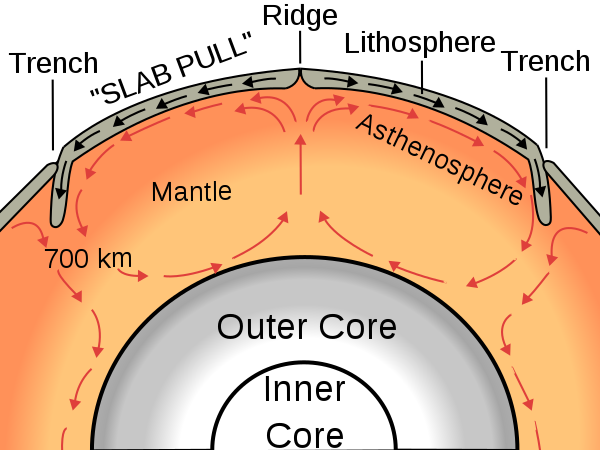
\includegraphics[width=0.30\textwidth]{introduzione/oceanic_spreading}
\end{wrapfigure}

La Terra è formata, nei primi 200 km di bordo esterno, da una zona chiamata \textit{litosfera}, di cui fa parte la \textit{crosta terrestre} con le terre emerse ed i fondali marini/oceanici. La \textit{litosfera} è divisa in parti, chiamate \textbf{placche tettoniche}, che "galleggiano" sul \textit{mantello superiore}. Queste placche sono continuamente spinte in direzioni diverse da \textit{moti convettivi} generati dalla temperatura elevata del nucleo. La zona di confine di queste placche viene chiamata \textbf{faglia}, e presenta diverse caratteristiche a seconda delle direzioni delle placche: se due placche si avvicinano, una delle due placche verrà immersa nel mantello sotto l'altra (\textit{subduzione}); se due placche si allontanano, una nuova parte della litosfera viene generata dalla roccia fusa proveniente dal mantello; infine, se due placche si muovo nella stessa direzione ma in senso opposto, siamo in presenza di \textit{margini di scorrimento}.

\begin{wrapfigure}[14]{r}{0.30\textwidth}
\caption{Mappa delle faglie italiane attive}
\label{fig:mappafaglie}
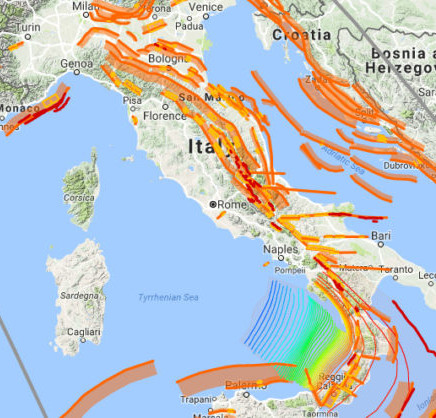
\includegraphics[width=0.30\textwidth]{introduzione/mappa_faglie_italiane2}
\end{wrapfigure}

Il movimento delle placche nei margini, tuttavia, non è libero da attrito: a seconda del materiale, della profondità e della conformazione della roccia presente nella faglia, la faglia stessa tende ad \textbf{opporsi} al movimento delle placche, accumulando energia da attrito. Quando si supera la massima forza d'attrito (per le caratteristiche ed il tipo di attrito attuato dalle due componenti rocciose), l'energia viene rilasciata repentinamente come energia meccanica (le cosiddette \textit{onde sismiche}) generando un \textit{terremoto} (o sisma).

Le onde sismiche generate da un terremoto si dividono in \textbf{Onde P} (onde di compressione, più veloci) e \textbf{Onde S} (onde trasversali, meno veloci delle onde P). Lo studio di queste due onde è importante per determinare non solo la distanza dell'ipocentro dal punto di osservazione, ma anche le caratteristiche del materiale sottostante: l'assenza di onde S è indice che tra il punto di osservazione e l'ipocentro è presente un liquido (come il magma, ad esempio), poiché le onde S non possono attraversare i liquidi\footnote{Poiché per un liquido il coefficiente di rigidità $\mu$ è nullo, la formula della velocità dell'onda S (con $\rho$ densità del materiale, in questo caso del liquido) $V_s = \sqrt{\mu \over \rho}$ è nulla, quindi l'onda S non attraversa i liquidi}.

\section{Analisi e misura dei terremoti}

Per misurare l'energia sprigionata da un evento sismico, individuare il punto di origine e altre caratteristiche dell'onda, si utilizzano i \textbf{sismometri}, apparati dotati di accelerometri molto precisi, filtri e amplificatori in grado di rilevare l'accelerazione sulle tre componenti (X-Y-Z) e produrre un \textit{sismogramma} (Figura \ref{fig:sismogramma}).

\begin{figure}[p]
\caption{La rete IV - Italian Seismic Network}
\label{fig:retesensori}
\centering
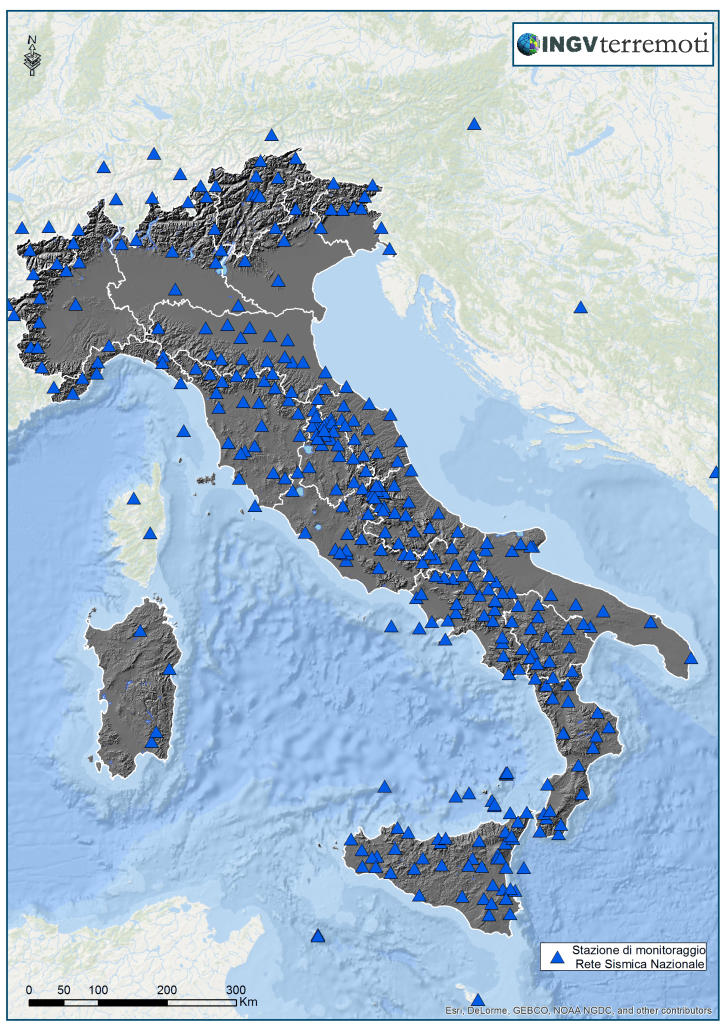
\includegraphics[width=\textwidth]{introduzione/rete_ingv}
\end{figure}

\begin{figure}[ht]
\caption{Esempio di sismogramma}
\label{fig:sismogramma}
\centering
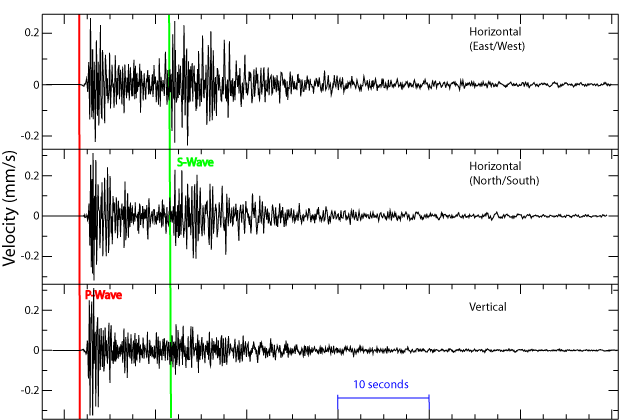
\includegraphics[width=10cm]{introduzione/seismogram}
\end{figure}

Attualmente nel mondo sono presenti diverse reti di rilevamento. Per l'Italia INGV riceve le informazioni da 27 reti sismiche (compresa la rete principale italiana \textit{IV - Italian Seismic Network}) per un totale di più di 800 sismometri (gran parte sul territorio nazionale, alcuni su paesi confinanti).

L'energia sprigionata viene misurata in \textbf{magnitudo} su una scala di valutazione chiamata \textbf{Richter}, mentre gli eventuali danni provocati vengono espressi in \textbf{intensità} del terremoto tramite valori della scala \textbf{Mercalli-Cancani-Sieberg}, o MCS \footnote{Le due scale non hanno un legame diretto: un terremoto di piccola magnitudo può fare molti danni in alcune situazioni (e quindi essere di elevata intensità MCS); viceversa un terremoto di magnitudo molto elevata può avere intensità molto bassa in altre situazioni.}.

Infine possiamo distinguere il punto di origine del terremoto sotto la superficie, chiamato \textbf{epicentro}, e la proiezione di questo punto sulla superficie terrestre, chiamato \textbf{ipocentro} \cite{introdseismo}.

\begin{figure}[ht]
\caption{Epicentro, ipocentro (o focus) e faglia (\textit{fault plane})}
\label{fig:epiipo}
\centering
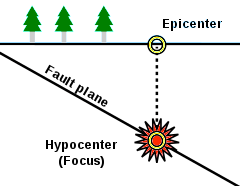
\includegraphics[scale=0.6]{introduzione/epicenter_diagram}
\end{figure}

\clearpage

\section{Prevedere o arginare i terremoti}

L'Italia è sottoposta, ogni giorno, ad un numero di terremoti nell'ordine del \textbf{centinaio di scosse}\footnote{Dati provenienti dal Centro Nazionale Terremoti: \url{http://cnt.rm.ingv.it/}}. Quasi tutti questi sismi sono classificati come \textit{microterremoti} (di magnitudo $<$ 2), poiché sono talmente deboli da essere percepibili solo dagli strumenti. Tuttavia, essendo l'Italia zona di confine tra la placca Europea e la placca Africana (con quest'ultima che si muove verso il Nord), la quantità di energia accumulata dalle faglie può generare terremoti in grado di infliggere ingenti danni.

Come in tutte le calamità naturali (e non), abbiamo diversi ambiti da considerare:
\begin{itemize}
\item la \textbf{prevenzione}, ovvero l'attuazione delle politiche in grado di minimizzare la probabilità che un evento accada e minimizzare il rischio all'accadere dell'evento
\item la \textbf{previsione}, ovvero l'utilizzo di tecniche e tecnologie che permettono di indicare \textit{quando un evento accadrà} (con una certa affidabilità)
\item la \textbf{gestione dell'emergenza} e del post-emergenza, ovvero delle azioni da mettere in campo durante e dopo il presentarsi di una calamità
\end{itemize}

Nella fattispecie dei terremoti, la \textbf{previsione} è tutt'ora materiale di studio da parte del mondo scientifico poiché risulta impossibile prevedere, allo stato attuale, quando e dove accadrà il prossimo sisma \cite{eqpred} \cite{alessamato}. Nel tempo, tuttavia, i vari dati raccolti riguardo ai terremoti hanno permesso di costruire delle mappe di pericolosità sismica\footnote{Pubblicate per la prima volta nel 2004 e poi aggiornate man mano: \url{http://zonesismiche.mi.ingv.it/}}, le quali indicano zone con maggiore probabilità di terremoti importanti, andando ad integrare le azioni di informazione e di formazione che fanno parte della \textbf{prevenzione}.

Nella gestione dell'emergenza possiamo riportare quello che avviene allo stato attuale all'accadere di un terremoto, rilevato (per l'Italia) dalla rete di sismometri di INGV: nel momento in cui un sisma viene percepito da un numero congruo di stazioni di rilevamento, il sistema effettua verifiche e calcoli e
\begin{itemize}
\item \textbf{entro due minuti}, è in grado di fornire una prima stima (non precisa) della magnitudo, dell'epicentro e della profondità; questi dati vengono comunicati alla Protezione Civile per una prima organizzazione dei soccorsi)
\item Successivamente, \textbf{entro 5 minuti} dal sisma, tutte le stazioni di rilevamento sono utilizzate per individuare le caratteristiche del terremoto in modo più preciso
\item Infine, \textbf{entro 30 minuti}, una verifica manuale da parte dei tecnici e ingegneri di INGV permette di avere il dato definitivo che viene di nuovo comunicato alla Protezione Civile e al pubblico\footnote{La pubblicazione avviene sul sito del Centro Nazionale Terremoti \url{http://cnt.rm.ingv.it/}, tramite le pagine ufficiali sui principali Social Network e attraverso i normali \textit{media}}.
\end{itemize}

\pagebreak

\section{Il progetto SeismoCloud}

\begin{wrapfigure}{r}{0.15\textwidth}
\centering
\label{fig:seismocloudlogos}

\includegraphics[width=0.15\textwidth]{app/seismocloud}

\includegraphics[width=0.15\textwidth]{logo-sapienza-mini}

\includegraphics[width=0.15\textwidth]{app/ingv}
\end{wrapfigure}

Il progetto SeismoCloud nasce dalla collaborazione dell'\textbf{Università degli Studi di Roma "La Sapienza"} e l'\textbf{Istituto Nazionale di Geofisica e Vulcanologia}. L'obiettivo di questo progetto è quello di implementare un sistema di \textbf{early warning} in \textit{crowdsourcing}\footnote{Un sistema si dice in \textit{crowdsourcing} quando i dati per il suo funzionamento vengono forniti dagli stessi utenti} per i terremoti, in grado di inserirsi nel \textit{gap} presente dal momento in cui il terremoto accade, al momento in cui INGV è in grado di individuarlo con l'affidabilità richiesta. Lo scopo del sistema quindi è di individuare i terremoti \textit{in tempo reale}, alla loro apparizione nell'ipocentro, ed \textbf{anticipare l'onda sismica nello spostamento} (dato che viaggia, mediamente, ad una velocità di 5 km/s), avvertendo la popolazione nel raggio di azione del terremoto. Questo sistema è chiamato, appunto, \textit{early warning}, poiché è in grado di fornire un avvertimento poco prima dell'evento sismico. \textbf{Il tempo tra l'avvertimento e l'arrivo della scossa varia in funzione della distanza}: partendo da un valore nullo all'epicentro, si può arrivare fino a 20 secondi di anticipo: questo, sommato al tempo che impiega una persona a comprendere che le oscillazioni sono effettivamente un terremoto (dato che l'arrivo dell'onda, sebbene veloce, è graduale), fornisce \textbf{tempo prezioso per mettersi in sicurezza} ed eventualmente lanciare automatismi in grado di rendere l'ambiente (azienda, casa, scuola) più sicuro (ad esempio, blocco della distribuzione del gas, messa in sicurezza degli ascensori, etc).

Già da un decennio alcuni luoghi più sensibili al terremoto si stanno dotando di infrastrutture di \textit{early detection}. Il primo Paese nel 2006 è stato il Giappone, con un sistema denominato \textbf{Earthquake Early Warning}, installato dalla \textbf{JMA} (Japan Meteorological Agency). Tale sistema è composto da 4325 sismometri su tutto il territorio giapponese \cite{jma}. Il funzionamento è il seguente: quando due o più sensori individuano una scossa di terremoto, il sistema invia degli avvisi immediati attraverso radio, TV e cellulari. L'efficacia\footnote{Per "efficacia" si intende la percentuale di allarmi emessi subito dopo l'individuazione di una onda-P aventi come magnitudo $\pm1$ il valore misurato per il terremoto} di questo sistema, misurata dallo stesso JMA sul territorio nazionale giapponese, varia dal 28\% al 76\% \cite{jma}.

Tuttavia comporre reti di \textit{early detection} molto accurate e molto rapide, con gli stessi sismometri installati per lo studio dei terremoti, è una operazione \textbf{complessa} oltre che \textbf{costosa}: si deve posizionare il sismometro nel terreno (a volte a decine di metri di profondità), si deve mantenere un collegamento stabile e affidabile alla rete di rilevamento oltre che l'energia per far funzionare gli apparati in loco. Ecco perché SeismoCloud affronta il problema con una soluzione \textbf{crowd-sourced}: quasi tutti gli smartphone moderni sono dotati di sensori in grado di rilevare le vibrazioni (oltre che la posizione geografica) in modo relativamente accurato\cite{eewapp}: questo permette ad ogni utilizzatore di un cellulare, tramite una app denominata \textbf{SeismoCloud}, di contribuire alla rilevazione dei terremoti. Inoltre, con l'esplosione dell'\textit{IoT}\footnote{\textit{Internet of Things}, letteralmente \textit{internet delle cose} è l'insieme dei piccoli dispositivi, che eseguono un gruppo di funzioni ristrette (ad esempio, accendi/spegni la luce), connessi alla rete Internet} ed il costo contenuto dell'hardware di questa categoria, reti hobbystiche e comunitarie (come ad esempio le Mesh Networks) possono contribuire in modo aperto e libero.

\pagebreak
%
%\begin{figure}[ht]
%\centering
%\label{fig:scsapp}
%\caption{Schermata principale dell'applicazione \textbf{SeismoCloud}}
%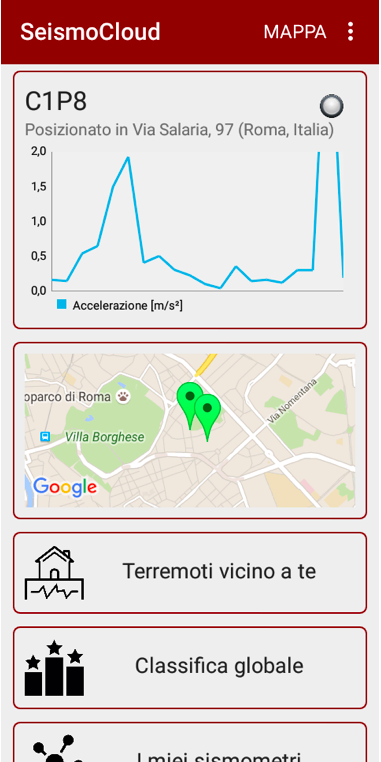
\includegraphics[width=0.5\textwidth]{app/main}
%\end{figure}
%
%\pagebreak

\section{Architettura della rete SeismoCloud}

Essendo un sistema in \textit{crowdsourcing}, i dati della rete provengono dagli utenti; sono disponibili applicazioni per smartphones (Android, iOS) e per dispositivi \textit{Internet of Things} (Arduino, NodeMCU, Raspberry PI) in grado di collezionare, con apposito sensore chiamato \textbf{accelerometro}, i dati di accelerazione nei tre assi (X, Y, e Z) del telefono (posizionati come indicato dalla figura \ref{fig:scsaxes}). La poca precisione di questi sensori (vedi tabella \ref{table:datisensori}), in relazione ai sensori delle reti sismiche ufficiali, non permette di conoscere le componenti importanti per lo studio puntuale e storico dei fenomeni (ad esempio la distanza tra le onde P e le onde S), tuttavia permette, con una certa affidabilità, di individuare la presenza di eventi sismici in atto se le misure singole dei vari dispositivi sono messe in relazione tra di loro.

\begin{table}[h]
\centering
\caption{Confronto tra l'accelerometro CMG-5T della rete IV (sismometro IV.LATB, posizionato a Latina) con l'accelerometro di uno smartphone ADXL345}
\label{table:datisensori}
\begin{tabular}{lll}
                    & \textbf{Frequenza massima (Hz)} & \textbf{Precisione (g)} \\
\textbf{CMG-5T} \cite{ivlatb} & 100 & $\pm 2.384 * 10^{-7}$ \\
\textbf{ADXL345} \cite{accelman}          & 50 & $\pm 3.91 * 10^{-3}$
\end{tabular}
\end{table}

Sebbene i valori siano così differenti, come si evince dalla tabella \ref{table:consumosensori}, poiché le onde sismiche hanno frequenze tra 0.1 e 15 Hz\footnote{Fonte: USGS, U.S. Geological Survey; \url{https://earthquake.usgs.gov/learn/facts.php}} la frequenza è adatta al rilevamento. La sensibilità, sebbene nettamente inferiore, è sufficiente ad individuare i terremoti in superficie \cite{finazzi}.

\begin{figure}[ht]
\centering
\label{fig:scsarch}
\caption{Architettura della rete SeismoCloud}
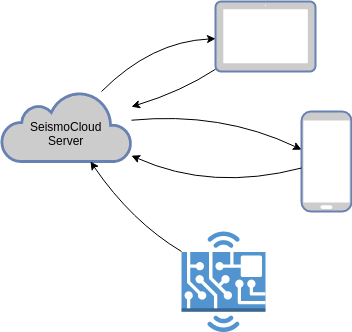
\includegraphics[width=0.8\textwidth]{introduzione/SeismoCloud_arch}
\end{figure}

Dal punto di vista utente, contribuire diventa rapido ed economico: una volta installata la \textit{app}, il sistema si avvia, acquisisce la posizione GPS ed entra a far parte della rete. Si è stimato che, per poter coprire un territorio come quello italiano occorrono dai 3000 ai 4000 sismometri, siano essi \textit{app} per cellulari o dispositivi fisici.

\section{Algoritmo di rilevamento}
\label{section:algoritmo}

Il funzionamento del sistema è il seguente: ogni dispositivo (smartphone o dispositivo \textit{IoT}) ha almeno due stati: \textbf{ALIVE} e \textbf{QUAKE}. Un dispositivo nello stato di \textbf{ALIVE} effettua una rilevazione dell'accelerazione su ogni asse ogni $20ms$, e viene calcolata la componente del vettore risultante mediante la formula~\ref{eq:vettoreris}. Il valore viene quindi confrontato con un valore di soglia calcolato (\ref{eq:soglia}) in modo da filtrare il rumore di fondo e, se la rilevazione risulta superiore alla soglia, il dispositivo informa il server comunicando l'attuale accelerazione rilevata, la posizione geografica ed il momento della rilevazione espresso in tempo UNIX\footnote{Il "tempo UNIX" è definito come il numero di secondi dallo \textit{UNIX Epoch Time}, ovvero dal 1 Gennaio 1970} (con precisione di $\pm1ms$), e successivamene passa allo stato di \textbf{QUAKE}.

\begin{equation} \label{eq:vettoreris}
Acceleration = \sqrt{Value(X)^2 + Value(Y)^2 + Value(Z)^2}
\end{equation}

\begin{equation} \label{eq:soglia}
Threshold = Mean + Variance * \sigma
\end{equation}

Il rilevamento, con l'algoritmo sopra citato, avviene in background rispetto all'attività utente: in questo modo si consente il multitasking sul dispositivo e si mantiene l'applicazione sempre attiva in modo trasparente per l'utente.

\begin{figure}[ht]
\centering
\caption{Posizionamento assi cartesiani in uno smartphone}
\label{fig:scsaxes}
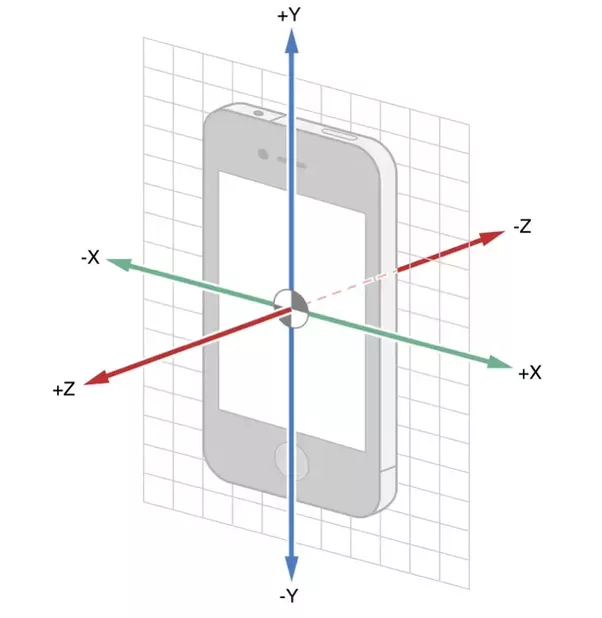
\includegraphics[width=0.5\textwidth]{introduzione/smartphone_axes}
\end{figure}


\begin{figure}[ht]

\begin{adjustbox}{addcode={\begin{minipage}{\width}}{
	\caption{Simulazione del terremoto dell'Aquila del 2009 - in rosso i sismometri simulati che hanno avvertito il terremoto, in viola le province avvertite (il punto è sul capoluogo ma rappresenta l'intera provincia) - Nella simulazione animata "l'onda" rappresentata dai Pin rossi è appena visibile quando le province (immediatamente) vengono avvertite dell'arrivo del terremoto}\label{fig:scssim}\end{minipage}},rotate=90,center}
      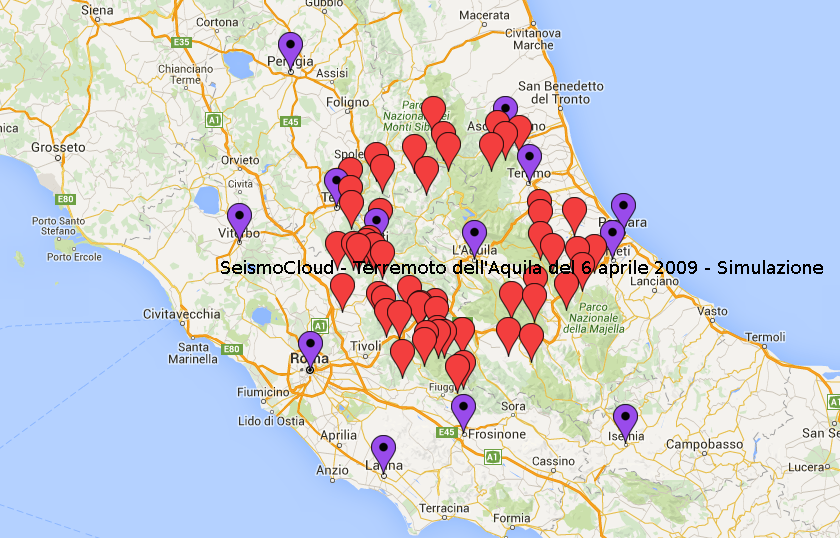
\includegraphics[width=1.2\textwidth]{introduzione/simulazione}
  \end{adjustbox}
\end{figure}


\begin{figure}[ht]

\begin{adjustbox}{addcode={\begin{minipage}{\width}}{
	\caption{Grafico dei dati estratti da un sensore SeismoCloud. La linea rossa rappresenta la soglia del dispositivo, le linee verdi, blu e azzurra rappresentano le eventuali soglie alternative calcolate con un valore moltiplicativo del server differente}\label{fig:scstrace}\end{minipage}},rotate=90,center}
      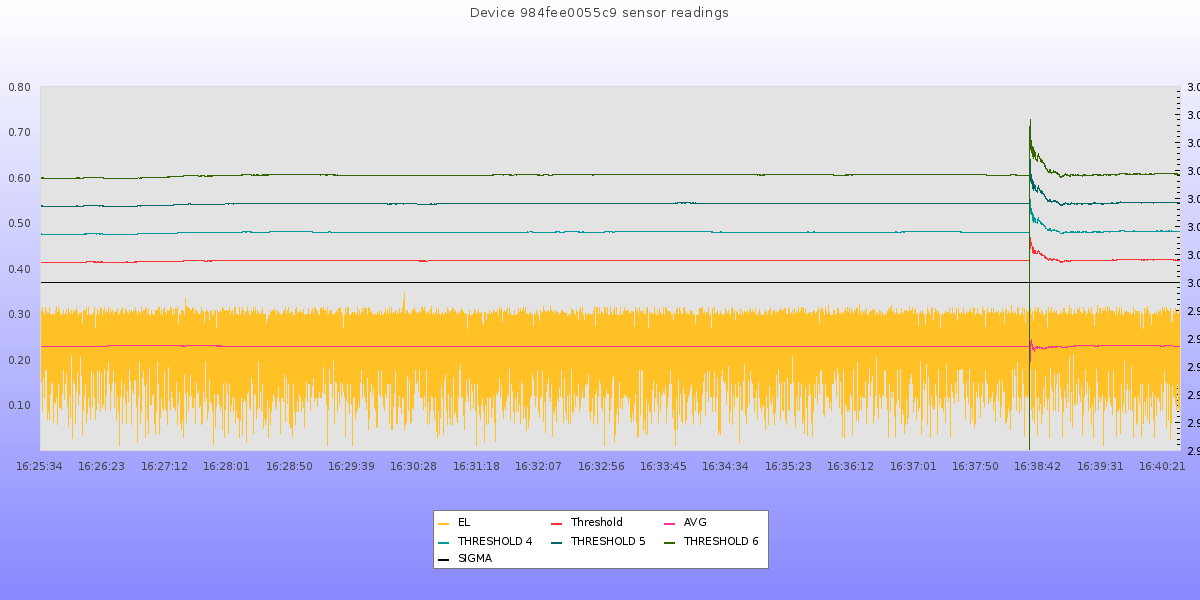
\includegraphics[width=1.2\textwidth]{database/984fee0055c9}
  \end{adjustbox}
\end{figure}

\chapter{Ottimizzazione energetica}

A differenza della vecchia generazione di cellulari, gli smartphones moderni fanno un uso intensivo delle risorse a bordo. In particolar modo, processori più potenti, nuove funzionalità hardware e software e multimedialità hanno reso gli smartphones moderni voraci di energia elettrica. Ecco perché è importante, quando si sviluppa codice per dispositivi \textit{mobile} (e, più in generale, per qualsiasi contesto non collegato alla griglia di distribuzione elettrica pubblica), utilizzare al meglio le capacità del dispositivo, pensando e scrivendo algoritmi \textit{battery-friendly}.

\section{I contesti di attivazione}
\label{section:contesti}

Il primo processo di ottimizzazione che è stato portato avanti riguarda i \textbf{contesti di attivazione}. Definiamo il \textbf{contesto di attivazione} come l'insieme delle variabili che rappresentano lo stato del telefono (come: stato batteria, attività utente, etc).

\paragraph{Versione base} Nella prima scrittura dell'algoritmo di rilevamento erano presenti solo due stati: \textbf{ALIVE} e \textbf{QUAKE}. All'accensione del servizio in background (avviato automaticamente dal sistema all'accensione del telefono), il telefono passava nello stato di \textbf{ALIVE} per effettuare le rilevazioni, per poi passare allo stato di \textbf{QUAKE} nel momento di una rilevazione sopra soglia. Chiaramente questo sistema prevedeva che il telefono rimanesse in orizzontale tutto il tempo. Questa prima versione è stata utilizzata in fase di test preliminare per valutare l'efficacia degli algoritmi di soglia e di rilevamento.

\begin{figure}[ht]
\centering
\label{fig:scs_sm0}
\caption{Diagramma degli stati con Alive e Quake}
\digraph[width=0.5\textwidth]{StateMachine0}{
rankdir=LR;
Quake->Alive [label="Quake motion reported"];
Alive->Quake [label="Quake motion detected"];
}
\end{figure}

\paragraph{Prima ottimizzazione} Poiché il telefono può essere in posizione non ottimale per il rilevamento, si è deciso di procedere all'attivazione del servizio solo quando il telefono si trova in \textbf{posizione orizzontale} (con le tecniche specificate nella sezione \ref{section:sensori}). Questa modifica permette di risparmiare le risorse, ed in particolar modo la batteria (tramite la diminuzione della pressione sulla CPU e memoria), quando il telefono è usato dall'utente oppure non poggiato su una superficie piana (ad esempio, il telefono si trova in una tasca oppure in una borsa). Per stabilire le soglie dei valori da considerare come "rotazione" si è stabilito un \textit{range} di rotazione assoluto rispetto al piano orizzontale, ed un offset di rotazione relativo. \textbf{Questo ci permette di individuare sia il posizionamento non favorevole del telefono, sia una sua rotazione o spostamento in modo repentino}. Quest'ultimo caso è importante perché ci ha permesso di ridurre al minimo i falsi positivi relativi all'azione dell'utente (ad esempio il prendere in mano il telefono) su un cellulare posizionato, fino a quel momento, in orizzontale. Abbiamo quindi introdotto un nuovo stato, lo stato di \textbf{MOVE}. La transizione da uno stato all'altro è determinata dai controlli fatti sui valori dei sensori.

\begin{listing}[H]
\caption{Codice di gestione della rotazione (alcune linee sono state accorpate per la stampa)}
\begin{minted}[mathescape,
               linenos,
               numbersep=5pt,
               gobble=0,
               fontsize=\small,
               frame=lines,
               framesep=2mm]{java}
boolean inRotation = Math.abs(gravity[2]) < gravityThreshold
		|| !(gravity[0] > -1 && gravity[0] < 1)
		|| !(gravity[1] > -1 && gravity[1] < 1);
if (isMoving)
	// Siamo in movimento - MOVE - valuto una transizione MOVE->FLAT
	if (accelerometerIntensity < 0.3 && !inRotation) {
		// I valori sono buoni per considerare la posizione come FLAT
		if (++countFlat > 5) {
			// Soglia di 5 valori OK per FLAT, passaggio a FLAT
			switchToMove(false); countFlat = movingLastMs = 0;
			seismometer.reset();
			// Informo il server che sono di nuovo OK
			WebApiInterface.alive(...);
		}
	} else countFlat = 0; // riparto da zero per MOVE->FLAT
else // Siamo in posizione stabile - FLAT - controllo se siamo in rotazione
	if (inRotation) {
		// Valori fuori scala per FLAT - transizione FLAT->MOVE
		goToMoving(); isQuake = 0;
		movingLastMs = System.currentTimeMillis();
	} else if (seismometer.tick(accelerometerIntensity)
			&& magneticValues[0] != 0 && magneticValues[1] != 0
			&& magneticValues[2] != 0) {
		// Calcolo la rotazione
		float[] rot = computeOrientation(); oldRotation = rotation;
		rotation = 1000*sqrt(rot[0]*rot[0]+rot[1]*rot[1]+rot[2]*rot[2]);
		deltaRot = (oldRotation==0.0d)?0.0d:abs(rotation-oldRotation);
		countFlat = 0;
		if (deltaRot > 75.0) {
			// il telefono e' in rotazione, quindi si va in MOVE
			goToMoving(); movingLastMs = System.currentTimeMillis();
		} else if (!inQuakeCondition) {
			// Niente rotazione pero' valore sopra soglia
			seismometer.addValueToAvgVar(accelerometerIntensity);
			Double d = Math.floor(System.currentTimeMillis()/1000D);
			WebApiInterface.terremoto(d.intValue(), location);
			magneticValues = new float[]{0, 0, 0};
			oldRotation = rotation = deltaRot = 0.0d;
			isQuake = System.currentTimeMillis();
			stopCause = StopCause.QUAKE;
		}
	} else {
		countFlat++;
		// Aggiorno la soglia
		if (!inQuakeCondition)
			seismometer.addValueToAvgVar(accelerometerIntensity);
		// Keep alive
		if (System.currentTimeMillis() - timerAlive > 15 * 60 * 1000) {
			WebApiInterface.alive(...);
			timerAlive = System.currentTimeMillis();
		}
	}
\end{minted}
\end{listing}

\begin{figure}[ht]
\centering
\label{fig:scs_sm1}
\caption{Diagramma degli stati con Alive, Quake e Move}
\digraph[width=\textwidth]{StateMachine1}{
Start [style=invis];
rankdir=LR;
Start->Alive [label="Service started"];
Quake->Alive [label="Quake motion reported"];
Alive->Quake [label="Quake motion detected"];
Alive->Move  [label="Rotation off-range"];
Move->Alive  [label="Rotation normal"];
}
\end{figure}

\paragraph{Seconda ottimizzazione} Una seconda ottimizzazione è stata apportata dallo spegnimento del servizio per un periodo stabilito quando il telefono si trova in uno stato non utile (\textit{MOVE} ad esempio). E' stato introdotto lo stato di \textbf{MOVE\_BACKOFF}, dove il servizio viene portato dopo un periodo di permanenza in \textit{MOVE}. Questo stato prevede lo \textbf{spegnimento} del servizio, con il rilascio di tutti i WakeLocks\footnote{Un "WakeLock" è un meccanismo di segnalazione, al sistema operativo Android, che permette di richiedere di lasciare attivi alcuni sottosistemi, come lo schermo od il chip WiFi - se nessuno richiede un WakeLock infatti, il cellulare va in uno stato di quiete per cui la CPU principale, il WiFi e altri chip vengono spenti}. Per decidere quando riattivare il servizio (e controllare se ci sono le condizioni per passare allo stato di \textit{ALIVE}) viene utilizzato un algoritmo di \textbf{backoff esponenziale}: al primo passaggio allo stato di \textit{MOVE\_BACKOFF} il tempo per il risveglio (e quindi il prossimo controllo) viene impostato a 30 secondi. Successivamente, se il controllo per il passaggio da \textit{MOVE} as \textit{ALIVE} fallisce (quindi rimaniamo dentro \textit{MOVE}) il tempo di \textit{MOVE\_BACKOFF} viene raddoppiato ogni volta, fino ad un massimo di 900 secondi.

In questo modo il servizio, durante il periodo di \textbf{MOVE\_BACKOFF}, non consuma risorse e non detiene nessun tipo di WakeLock, permettendo quindi al telefono di andare in \textit{stand-by} e gestire il sistema come se SeismoCloud non fosse installato. \textbf{Il consumo determinato dalla nostra app mentre il telefono è in uso, oppure in posizione non orizzontale, è zero}. Il risveglio invece è gestito dal sistema operativo \textbf{Android}, il quale gestisce in modo ottimizzato gli interrupt basati sul tempo (come questo per la riattivazione del servizio), spesso (sui telefoni che lo supportano) con un chip dedicato a consumo molto ridotto.

\begin{figure}[ht]
\centering
\label{fig:scs_sm2}
\caption{Diagramma degli stati con Alive, Quake, Move e Move\_Backoff}
\digraph[width=\textwidth]{StateMachine2}{
rankdir=LR;
{
Quake->Alive [label="Quake motion reported"];
Alive->Quake [label="Quake motion detected"];
Alive->Move  [label="Rotation off-range"];
Move->Alive  [label="Rotation normal"];
Move_Backoff->Move  [label="Interrupt (timeout)"];
Move->Move_Backoff  [label="Persistent Move state"];
}
{
rankdir=TB;
Start [style=invis];
Start->Alive [label="Service started"];
}
{
rankdir=TB;
rank=min;
Move_Backoff;
}
}
\end{figure}

\paragraph{Controllo della localizzazione} Una ulteriore ottimizzazione è stata l'introduzione del controllo sulla effettiva disponibilità del segnale GPS o dalla localizzazione da rete (utilizzata qualora non sia presente il GPS sul dispositivo, oppure non sia abilitato o ancora non sia presente il segnale satellitare): sia in fase iniziale, sia durante il funzionamento (stato \textbf{ALIVE}), il sistema controlla l'effettiva presenza di una localizzazione valida (sia essa il GPS o una posizione acquisita tramite rete cellulare). Questo permette di individuare diverse situazioni a noi sfavorevoli:

\begin{itemize}
\item \textbf{Disattivazione del sensore di localizzazione} da parte dell'utente (tramite apposita opzione di Android) oppure perdita del segnale
\item \textbf{Spostamento} del telefono (inteso come identificazione dello spostamento geografico dell'utente, ad esempio quando si muove in auto)
\end{itemize}

In entrambi i casi il servizio non è più in grado di fare affidamento alla posizione memorizzata, dunque entra nello stato di \textbf{MOVE\_BACKOFF}, dove continuerà ad essere fino alla riaccensione del sensore di localizzazione (nel primo caso) o ad una posizione valida e fissa (nel secondo caso). Questo ha permesso di ridurre, come da test effettuati, il consumo di batteria in particolari condizioni: ad esempio posizionare il telefono sul cruscotto di una automobile, o su di un tavolino del treno, avrebbe comportato l'attivazione del servizio a causa della posizione orizzontale, tuttavia i dati di accelerazione sarebbero stati ovviamente inutili ai fini dell'indentificazione del terremoto. Dunque, \textbf{con questa nuova aggiunta il sistema è in grado di rilevare questi casi} e si pone nello stato corretto.

Poiché la precisione della localizzazione via rete cellulare è molto variabile (dai pochi metri a decine di km), è stato stabilito di non considerare localizzazioni via rete cellulare che hanno un errore maggiore di $\pm250$ metri.

\paragraph{Controllo della connessione dati} Un altro fattore importante per una buona rilevazione è la presenza della connessione di rete (Wi-Fi o rete cellulare). Qualora venga a mancare la connessione Internet non si potrà avvertire per tempo il server: il sistema è quindi portato nella posizione di \textbf{MOVE\_BACKOFF} con l'algoritmo sopra citato. Questo permette di risparmiare batteria quando il segnale è assente.

Per l'identificazione dello stato di \textit{mancanza della connessione dati} si sono utilizzate le API di Android: il sistema operativo infatti fornisce già informazioni riguardo ai cambimenti di stato della connessione attraverso il \textit{dispatch} di un evento informativo (denominato ``\textit{CONNECTION\_CHANGED}") la quale scatena l'esecuzione del codice \ref{listing:connchange}.


\begin{listing}[H]
\caption{Codice eseguito al cambio di stato della connettività a bordo del telefono}
\label{listing:connchange}
\begin{minted}[mathescape,
               linenos,
               numbersep=5pt,
               gobble=0,
               frame=lines,
               framesep=2mm]{java}
ConnectivityManager cManager =
	(ConnectivityManager) ctx.getSystemService(CONNECTIVITY_SERVICE);
NetworkInfo mWifi = cManager.getNetworkInfo(ConnectivityManager.TYPE_WIFI);
NetworkInfo mData = cManager.getNetworkInfo(ConnectivityManager.TYPE_MOBILE);

if (mWifi.isConnected() || mData.isConnected())
	MySeismoService.startService(context);
else
	MySeismoService.stopService(context);
\end{minted}
\end{listing}

\paragraph{La batteria} Infine, è stata fatta una analisi sulla batteria e sul consumo. In prima istanza è stato considerato lo status di "\textbf{risparmio energia}" che Android attiva nel momento in cui la batteria raggiunge un valore prefissato (in genere, a meno di cambiamenti fatti dall'utente, il valore è il 15\% della capacità). Grazie ad un \textit{handler} viene intercettato questo evento e viene posto il servizio nella fase di \textbf{MOVE\_BACKOFF} indipendentemente dalle condizioni favorevoli sopra citate.

Una seconda analisi ha riguardato il sotto-sistema \textbf{Doze} introdotto in \textbf{Android 6.0} \cite{doze}: l'obiettivo di \textit{Doze} è di bloccare (a schermo spento) l'esecuzione delle applicazioni e disattivare le connessioni esterne, a scopo di risparmio energetico, anche se hanno ottenuto WakeLocks o altri meccanismi che tengono accesa la CPU. Poiché, in molti casi, queste applicazioni eseguono in background attività \textit{rimandabile}, \textbf{il sistema effettua delle accensioni ad intervalli regolari}, chiamate \textit{finestre di manutenzione}: in queste finestre temporali le app vengono riaccese ed il sistema si riconnette alle reti mobili. Ovviamente nel nostro caso questo rappresenta un problema, poiché la rilevazione deve avvenire sempre. Viene quindi richiesto al sotto-sistema \textit{Doze}, in fase di avvio, l'inserimento della nostra App nella lista delle eccezioni per questo algoritmo (tramite le API di Android).

Dopodiché si è provveduto ad effettuare uno studio approfondito meglio specificato nella sezione \ref{section:curvascarica}.

\paragraph{Conclusioni} Abbiamo quindi definito una serie di variabili che compongono il nostro \textbf{contesto di attivazione}, ovvero:

\begin{itemize}
\item Rotazione/posizione favorevole o no alla lettura del dato
\item Persistenza della posizione sfavorevole nel tempo
\item Presenza o meno della localizzazione GPS
\item Presenza o meno di uno spostamento geografico
\item Presenza o meno della rete Internet
\item Status di risparmio energetico del sistema operativo (capacità batteria rimanente)
\end{itemize}

Questa definizione ci permette di stabilire, come abbiamo fatto, una istanza del contesto per la quale è favorevole attivare il servizio (localizzazione presente, posizione orizzontale, etc.), permettendo così un risparmio notevole (come evidenziato dalla tabella \ref{table:tempoutilizzo} e dalla figura \ref{fig:usagechart}). Nella figura \ref{fig:scs_sm3} invece è rappresentato il diagramma degli stati dopo le ottimizzazioni esposte. L'impatto di queste e successive ottimizzazioni sulla batteria è possibile vederlo nella figura \ref{fig:batterychart} a pagina \pageref{fig:batterychart}.

\begin{table}[h]
\centering
\begin{tabular}{lllll}
& \textbf{Servizio attivo} & \textbf{Servizio inattivo} & \textbf{Telefono spento} &  \\
Algoritmo originale   & 18 ore e 24 min  & mai              & 5 ore 36 min &  \\
Algoritmo ottimizzato & 6 ore e 36 min   & 11 ore e 48 min  & 5 ore 36 min &
\end{tabular}
\caption{Tempo di utilizzo delle risorse (media giornaliera)}
\label{table:tempoutilizzo}
\end{table}

\begin{figure}[ht]
\centering
\caption{Diagramma degli stati per i contesti di attivazione}
\label{fig:scs_sm3}
\digraph[width=\textwidth]{StateMachine3}{
rankdir=TB;
{
Quake->Alive [label="Quake motion reported"];
Alive->Quake [label="Quake motion detected"];
Alive->Move  [label="Rotation off-range"];
Move->Alive  [label="Rotation normal"];
Move_Backoff->Move  [label="Interrupt (timeout)"];
Move->Move_Backoff  [label="Persistent Move state"];
Alive->Move_Backoff  [label="Location unavailable/move"];
Alive->Move_Backoff  [label="Android Power safe mode"];
Alive->Move_Backoff  [label="Internet unavailable"];
}
{
Start [style=invis];
Start->Alive [label="Service started"];
}
{
rank=sink;
Move_Backoff;
}
}
\end{figure}

\begin{figure}[ht]
\centering
\caption{Comparazione (valori medi in un giorno) dell'utilizzo delle risorse CPU e sensori da parte degli algoritmi con (\textit{Context-based}) e senza (\textit{Basic}) contesto di attivazione: si può notare come il tempo di inattività in blu (\textbf{MOVE\_BACKOFF}) sia una porzione notevole del tempo totale}
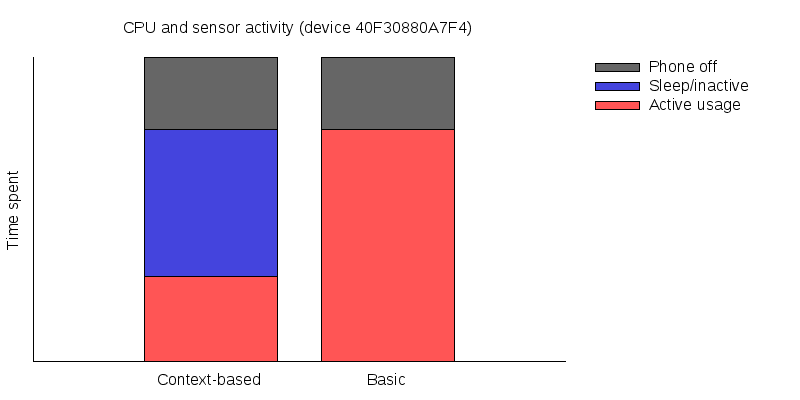
\includegraphics[width=\textwidth]{database/usageplot}
\label{fig:usagechart}
\end{figure}

\clearpage

\section{La comunicazione con il front-end}
\label{section:frontend}

Sebbene l'ottimizzazione del front-end (nell'uso delle risorse e nell'interazione con l'utente) non sia lo scopo di questa tesi, ci sono alcuni aspetti inseriti nel funzionamento interno dell'interfaccia grafica che prevedono uno scambio di informazioni (e, a volte, interazioni più vicolanti) con il servizio di rilevamento che gira in background.

\paragraph{Un requisito di HCI} Nello sviluppo dell'applicazione, prima delle ottimizzazioni citate qui, sono stati effettuati alcuni studi di \textit{Human-Computer Interaction}. Questi studi avevano come obiettivo migliorare la comunicazione con l'utente riguardo al concetto di "contributo nella rilevazione", e quindi era stato stabilito di inserire, nella schermata principale dell'applicazione, un box contenente il grafico dato dai valori di accelerazione (formula~\ref{eq:vettoreris} pagina \pageref{eq:vettoreris}) nel tempo. Lo scopo di questo box è di mostrare all'utente quello che avviene e qual è lo stato del servizio di rilevamento che gira in background.

\begin{figure}[ht]
\centering
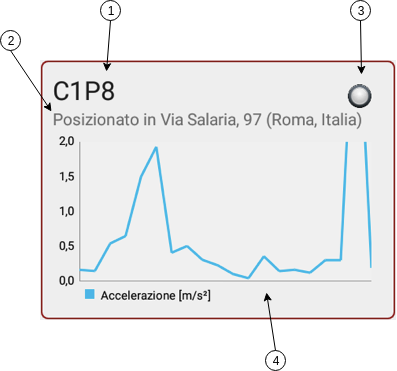
\includegraphics[width=0.7\textwidth]{app/activitychart2}
\caption{Porzione della schermata principale con il grafico del segnale dell'accelerometro: \textbf{1}: nome del sismometro (scelto dall'utente); \textbf{2}: Posizione georeferenziata; \textbf{3}: Indicatore di stato, verde: servizio attivo, rosso: vibrazione rilevata, grigio: servizio spento; \textbf{4}: Grafico del segnale dell'accelerometro}
\label{fig:activitychart}
\end{figure}

\paragraph{Adeguamento del codice} Dalle modifiche fatte per i contesti di attivazione (sezione \ref{section:contesti}) abbiamo alcune informazioni in più rispetto a prima, la più importante è lo stato del servizio di rilevamento. Per poter mostrare lo stato del servizio all'utente, è stato aggiunto un indicatore di stato (punto \textbf{3} figura \ref{fig:activitychart}) ed è stato inserito un testo descrittivo al posto del grafico nei seguenti casi:

\begin{itemize}
\item Servizio in stato di \textbf{MOVE}, con l'indicazione per l'utente di poggiare il telefono su una superficie orizzontale
\item Servizio in \textbf{MOVE\_BACKOFF} in caso di localizzazione o rete assente, con il testo relativo
\end{itemize}

Con le nuove ottimizzazioni inserite nei paragrafi precedenti, tuttavia, \textbf{il servizio non è sempre disponibile}: ad esempio in caso di batteria bassa (o sotto la soglia di scarica, sezione \ref{section:curvascarica}), o più semplicemente quando l'utente apre la app mentre ha il telefono in mano, il servizio risulterà fermo (per effetto dei \textbf{contesti di attivazione}, sezione \ref{section:contesti}). Poiché è importante che il servizio abbia un funzionamento coerente con i criteri di risparmio energetico che ci siamo prefissati, ma nello stesso tempo è importante fornire all'utente una informazione utile, è stata introdotta anche la seguente modifica, ai contesti di attivazione sopra citati, che include questi vincoli:

\begin{itemize}
\item Il passaggio da \textbf{MOVE} a \textbf{MOVE\_BACKOFF}, nei casi di \textbf{batteria bassa} (sotto la curva di scarica\footnote{Vedi sezione \ref{section:curvascarica}} o $<= 15\%$) o di \textbf{permanenza nello stato di MOVE}, avviene solo se la app è chiusa (ed è quindi attivo solo il servizio in background)
\item Se il servizio è spento (è già in \textbf{MOVE\_BACKOFF}) viene attivato
\end{itemize}

In sostanza, se l'utente \textbf{sceglie volontariamente} di avere l'informazione sul servizio, tale servizio deve essere attivo (se possibile, ovvero a meno di mancanza di rete/localizzazione).

\paragraph{Test di utilizzo} Diversi test di HCI, effettuati prendendo un campione di utenti rappresentativo, hanno confermato la validità di queste modifiche: la comunicazione con l'utente era rimasta pressoché invariata rispetto all'informazione fornita già in precedenza, con l'aggiunta utile degli stati del servizio tramite l'indicatore colorato ed il testo presente al posto del grafico nei casi sopra citati.

\section{I sensori}
\label{section:sensori}

Ogni modello di smartphone Android è dotato di un numero variabile di sensori, a seconda del produttore e della fascia di prezzo in cui si vuole inserire il dispositivo. Ogni sensore è in grado di misurare un particolare fattore esterno e/o interno al telefono. Alcuni sensori sono \textit{virtuali}, ovvero sono elaborazioni software dei dati provenienti da più sensori \textit{hardware}. Mentre i modelli \textit{top} di gamma hanno un numero impressionante di sensori (ad esempio il Samsung S4 è dotato di ben 34 sensori - virtuali e non - accessibili all'utente), altri telefoni hanno solo alcune tipologie di sensori.

\paragraph{Di cosa abbiamo bisogno} Il servizio della App SeismoCloud deve individuare le vibrazioni, quindi sicuramente è necessario l'\textbf{accelerometro}. Inoltre deve individuare, come abbiamo visto nel capitolo precedente, quando si trova poggiato con una inclinazione non utile per la rilevazione: per questo abbiamo bisogno del \textbf{giroscopio}. Inizialmente il codice fu scritto per questi due sensori, ma effettuando i test della applicazione abbiamo scoperto che molti telefoni di fascia "economica" sono sprovvisti del giroscopio. Poiché questi modelli di telefono sono i più diffusi, è stato effettuato uno studio per capire come poter ovviare al problema.

\paragraph{La fascia economica} Il problema della mancanza del giroscopio probabilmente è molto conosciuto agli sviluppatori Android, i quali hanno messo a disposizione una libreria che sfrutta un altro sensore, diffuso tanto quanto l'accelerometro: il \textbf{magnetometro}. Grazie ai valori letti dal magnetometro e dall'accelerometro, è possibile calcolare l'attuale rotazione del telefono (rispetto al piano orizzontale).

\begin{listing}[H]
\caption{Porzione di codice che calcola la rotazione in base ai dati del magnetometro e dell'accelerometro grazie alla chiamata API alla libreria \texttt{SensorManager} di Android}
\begin{minted}[mathescape,
               linenos,
               numbersep=5pt,
               gobble=0,
               frame=lines,
               framesep=2mm]{java}
private synchronized float[] computeOrientation() {
   float[] rotationMatrix = new float[16];
   float[] iMatrix = new float[16];
   float[] orientation = new float[3];
   // "gravity" contiene i valori dell'accelerometro
   // "magneticValues" contiene i valori del magnetometro
   if (SensorManager.getRotationMatrix(rotationMatrix, iMatrix,
                                       gravity, magneticValues)) {
      SensorManager.getOrientation(rotationMatrix, orientation);
   }
   return orientation;
}
\end{minted}
\end{listing}

\paragraph{Alla ricerca dell'ottimizzazione} Poiché il magnetometro e l'accelerometro forniscono un dato affidabile quanto basta per rilevare la rotazione sul piano orizzontale del telefono, e poiché la frequenza di rilevazione del magnetometro è impostabile (al contrario del giroscopio), si è deciso di procedere con un tentativo di ottimizzazione che includesse due fasi nella fase \textbf{ALIVE} (fase di rilevamento dei valori dell'accelerometro): sono state introdotte le fasi \textbf{ALIVE\_SLOW} e \textbf{ALIVE\_FAST}. Ogni fase registrava sensori differenti con frequenze differenti:

\begin{itemize}
\item \textbf{ALIVE\_SLOW}: registrati \textbf{magnetometro} e \textbf{accelerometro} con tempi di rilevazione di $100ms$
\item \textbf{ALIVE\_FAST}: registrati \textbf{giroscopio}, se presente, altrimenti \textbf{magnetometro}, e \textbf{accelerometro} con tempi di rilevazione di $20ms$
\end{itemize}

Inizialmente veniva attivata la fase \textbf{ALIVE\_SLOW}. Successivamente, ad una attività del magnetometro sopra soglia, il servizio passava allo stato di \textbf{ALIVE\_FAST} e controllava il dato del giroscopio (se presente, altrimenti di nuovo del magnetometro).

\begin{figure}[ht]
\centering
\caption{Diagramma degli stati per \textbf{ALIVE\_FAST} e \textbf{ALIVE\_SLOW}}
\label{fig:scs_sm4}
\digraph[width=\textwidth]{StateMachine4}{
rankdir=LR;
Start [style=invis];
Start->Alive_Slow [label="Service started"];
Alive_Fast->Alive_Slow [label="No significant rotation detected"];
Alive_Slow->Alive_Fast  [label="Significant rotation detected"];
}
\end{figure}

L'ipotesi era che questa diminuzione di frequenza fosse apprezzabile, sia dal punto di vista del carico sulla CPU, sia dal punto di vista del carico della batteria.

\paragraph{Test finali e conclusioni} Tuttavia, successivi test hanno rivelato come questa differenza ipotizzata tra le due frequenze di lettura sia praticamente nulla. Inoltre, la mancanza del giroscopio in alcuni telefoni aveva significato scrivere più codice per gestire tutti i casi. Infine, una indagine più approfondita dal punto di vista energetico ha svelato\footnote{\url{http://www.edn.com/design/sensors/4431747/Lower-power-and-cost-for-Android-device-motion-sensing-using-mCube-s-iGyro-}} \footnote{\url{https://www.sparkfun.com/pages/accel_gyro_guide}} che \textbf{il giroscopio ha un consumo enormemente maggiore rispetto all'accelerometro e al magnetometro}, i quali tra l'altro risultano spesso integrati in un solo chip (tabella \ref{table:consumosensori}). Si è quindi deciso di procedere eliminando il requisito del giroscopio e di mantenere solo una fase di \textbf{ALIVE} contenente la registrazione dei sensori \textbf{accelerometro} e \textbf{magnetometro} alla velocità stabilita.

\begin{table}[h]
\centering
\caption{Comparazione sul consumo delle tipologie di sensori più comuni per le due tipologie}
\label{table:consumosensori}
\begin{tabular}{lllll}
& \textbf{In fase di misura} & \textbf{Stand-by} & \\
Accelerometro + Magnetometro \\
ADXL345\cite{accelman} & $40 \mu A$ & $0.1 \mu A$ &  \\
Giroscopio \\
L3G4200D\cite{gyroman} & $6.1mA$ & $0.2mA$ &
\end{tabular}
\end{table}

\section{La curva di scarica}
\label{section:curvascarica}

Una risorsa molto importante, dal punto di vista degli utenti, è la batteria: mentre i vecchi telefoni avevano una autonomia di giorni se non settimane, i nuovi smartphones spesso richiedono una o più ricariche al giorno. L'obiettivo quindi è quello di portare il servizio di rilevamento dell'applicazione SeismoCloud ad impattare il meno possibile sul consumo totale, anche sacrificando periodi di rilevazione. Il motivo di questa scelta è semplice: un impatto ridotto dal punto di vista energetico può portare l'applicazione ad essere installata su più dispositivi, compensando il tempo di attività che verrebbe a mancare con l'introduzione dell'algoritmo esposto in questa sezione.

\paragraph{La curva di scarica} In parte, le ottimizzazioni già presentate nella sezione \ref{section:contesti} hanno portato ad un risparmio energetico; tuttavia si è voluto studiare un sistema più "\textit{aggressivo}" per portare i consumi al minimo possibile. Sono partito quindi da quello che è il principale requisito per l'utente: \textbf{il telefono deve arrivare a fine giornata}, ovvero nessuna applicazione deve consumare così tanto da rendere il telefono scarico prima di avere una fonte di energia.

Poichè in quasi tutti i casi le persone si trovano in un luogo con corrente elettrica per cena, facendo una rapida analisi sui dati presenti sul \textit{database} è stato identificato, come \textit{target}, una \textbf{carica residua del 15\% alle ore 20:00}, partendo dal 100\% alle ore 08:00. E' stata quindi calcolata una curva lineare di scarica, con lo scopo di tenere il servizio attivo solo quando è sopra la soglia (alla figura~\ref{fig:expectedchart} è possibile vedere una simulazione del comportamento atteso per la curva di scarica). Inoltre è stato deciso, grazie sempre ai dati presenti nel \textit{database}, che i valori convenienti per la carica attesa della batteria sono il 100\% prima delle 8 di mattina (dato che molti ricaricano lo smartphone durante la notte) ed il 15\% per le ore successive alle 20 di sera.

\pagebreak

\begin{equation}
\gamma = {85 \over 720}
\end{equation}

\begin{equation}
\lambda = \text{hour} * 60 + \text{minutes}
\end{equation}

\begin{equation}
	\\
    Threshold =
    \begin{cases}
        100 & \text{if hour} < 8\\
        15 & \text{if hour} > 20\\
        {100 - ((\lambda - 480) * \gamma)} & \text{otherwise.}
    \end{cases}
\end{equation}

Dove:
\begin{itemize}
\item $\gamma \in Z^+$: \textit{rate} di perdita della capacità della batteria per minuto nella fascia 8-20
\item $\lambda \in N^+$: numero di minuti a partire dalla mezzanotte del giorno attuale
\item $Threshold \in Z^+$ : la capacità della batteria (in percentuale) prevista per l'orario attuale
\end{itemize}

\begin{figure}[ht]
\centering
\caption{Comportamento atteso: la carica del cellulare (verde, in questo caso simulata) non deve mai scendere sotto la curva di scarica calcolata (rosso)}
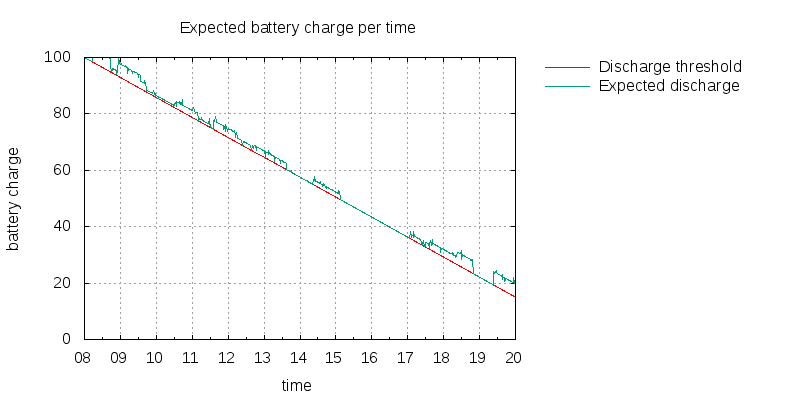
\includegraphics[width=\textwidth]{database/expectedplot}
\label{fig:expectedchart}
\end{figure}

Dopo averla applicata sui dispositivi di test, abbiamo subito notato un cambiamento notevole: nonostante un tempo di attività leggermente inferiore a causa dei distacchi per rispettare la soglia (cosa che, ovviamente, varia da telefono a telefono a seconda della capacità della batteria, delle applicazioni installate, dell'hardware del telefono e dell'utilizzo), il consumo evidenziato dai dati sul \textit{database} è nettamente migliore, come mostrato nella figura \ref{fig:batterychart}.

\begin{figure}[ht]

\begin{adjustbox}{addcode={\begin{minipage}{\width}}{
	\caption{Capacità residua batteria (media) prima e dopo l'ottimizzazione: \textbf{Basic} rappresenta l'algoritmo di base senza ottimizzazioni, \textbf{Context-based alg} rappresenta l'algoritmo che utilizza solo i contesti di attivazione, mentre \textbf{Discharge-curve alg} rappresenta l'algoritmo corrente, che sfrutta sia i contesti di attivazione che la curva di scarica}\label{fig:batterychart}\end{minipage}},rotate=90,center}
      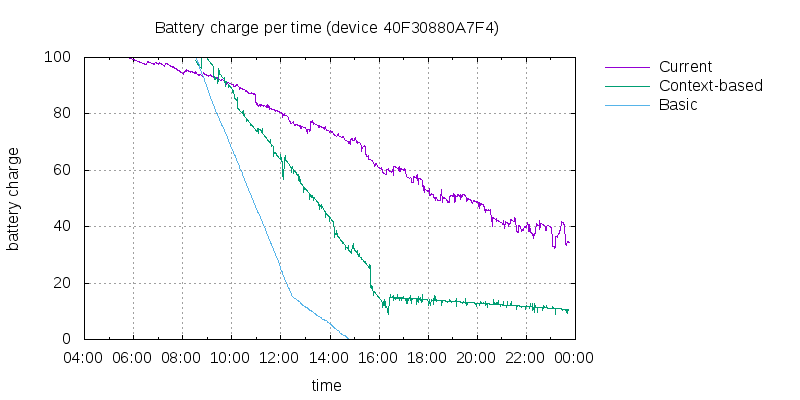
\includegraphics[width=\textwidth]{database/batteryplot}
  \end{adjustbox}
\end{figure}

\clearpage

\begin{listing}[H]
\caption{Porzione di codice che calcola la curva di scarica e indica se procedere o no con il servizio}
\begin{minted}[mathescape,
               linenos,
               numbersep=5pt,
               gobble=0,
               frame=lines,
               framesep=2mm]{java}
// Orario di inizio
private static final Double T0 = 8 * 60.0;
// Orario di fine
private static final Double T1 = 20 * 60.0;
// Carica iniziale
private static final Integer B0 = 100;
// Ratio di scarica
private static final Double R0 = (100.0 - 15.0) / (T1 - T0);

/**
 * Calcola il valore atteso della batteria all'orario corrente
 */
@NonNull
public static Double expectedBattery() {
	Calendar c = Calendar.getInstance();
	if (c.get(Calendar.HOUR_OF_DAY) < 8) {
		return 100.0;
	}
	Integer Tx = c.get(Calendar.HOUR_OF_DAY) * 60 + c.get(Calendar.MINUTE);
	return Math.floor(B0 - ((Tx - T0) * R0));
}

/**
 * Controlla se ci sono le condizioni per proseguire
 * (caricabatterie collegato oppure valore batteria sopra curva)
 */
public static boolean shouldProceedWithService(Context ctx) {
	if (BatteryLevelReceiver.isPowerSupplyConnected(ctx)) {
		return true;
	}
	Float now = Utils.getBatteryLevel(ctx);
	return now == 0 || (expectedBattery() <= now && now > 15.0);
}
\end{minted}
\end{listing}

\chapter{Ottimizzazione della rete}

Nell'ambiente \textit{mobile} un problema fondamentale con cui gli sviluppatori di \textit{app} si devono confrontare è l'affidabilità e le caratteristiche della connessione alla rete Internet. Su un dispositivo Android, sia esso smartphone o tablet, la connessione può arrivare tramite una rete Wi-Fi (IEEE 802.11a/b/g/n), oppure tramite rete cellulare attraverso reti che vanno dalla seconda generazione (EDGE) alla quarta generazione (LTE). La differenza notevole di caratteristiche tra le tecnologie, unita alla copertura non omogenea delle varie reti, obbliga gli sviluppatori a prendere delle decisioni implementative che siano in grado di sopportare e/o recuperare dalle mancanze temporanee dovute al \textit{roaming} sia tra reti mobile, es. tra HDSPA e LTE, sia con il Wi-Fi.

\section{Message Queue Telemetry Transport}
\label{section:mqtt}

\paragraph{Obiettivo} Lo studio di questa sezione si è concentrato sul come ridurre al minimo i problemi legati alla perdita di dati durante il roaming, in particolare per i dati del servizio di rilevamento. Lo status attuale, al momento dell'analisi, prevedeva l'utilizzo di chiamate HTTP (ovvero che sfruttavano l'\textit{HyperText Transfer Protocol}\footnote{L'HyperText Transfer Protocol è lo standard per la navigazione web: i browser (Mozilla Firefox, Google Chrome) sono esempi di "client HTTP"}) verso il server SeismoCloud per le API del servizio in background, con il passaggio dei dati (da e verso il telefono) in queste richieste.

\begin{listing}[H]
\caption{Richiesta HTTP classica per la API "alive.php"}
\label{listing:httpreq}
\begin{minted}[mathescape,
               linenos,
               numbersep=5pt,
               gobble=0,
               frame=lines,
               framesep=2mm]{http}
POST /seismocloud/alive.php HTTP/1.1
User-Agent: Mozilla/5.0 (X11; Linux x86_64; rv:54.0) Gecko/20100101 Firefox/54.0
Host: www.sapienzaapps.it
Content-Type: application/x-www-form-urlencoded
Content-Length: 57
Accept-Language: it-it
Accept-Encoding: gzip, deflate, br
Connection: keep-alive

deviceid=0123456789&lat=0&lon=0&model=android&version=2.2
\end{minted}
\end{listing}

\begin{listing}[h]
\caption{Risposta classica HTTP alla chiamata "alive.php"}
\label{listing:httpresp}
\begin{minted}[mathescape,
               linenos,
               numbersep=5pt,
               gobble=0,
               frame=lines,
               framesep=2mm]{http}
HTTP/1.1 200 OK
Date: Sat, 22 Jul 2017 22:38:34 CEST
Content-Type: text/html; charset=UTF-8
Content-Encoding: UTF-8
Content-Length: 79
Last-Modified: Sat, 22 Jul 2017 22:38:34 CEST
Server: Apache/1.3.3.7 (Unix)
ETag: "3f80f-1b6-3e1cb03b"
Accept-Ranges: bytes
Connection: close

{"sigma":2,"trace":0,"server":"www.sapienzaapps.it","ntpserver":"pool.ntp.org"}
\end{minted}
\end{listing}

Come è ben visibile da una richiesta HTTP di una delle \textit{Application Program Interface} di comunicazione smartphone-server (listato \ref{listing:httpreq}) e dalla relativa risposta (listato \ref{listing:httpresp}), molte di queste informazioni sono ridondanti ed inutili: la struttura \textit{human-readable} di HTTP è ovviamente un vantaggio in fase di scrittura delle implementazioni, o in fase di debug dei software, \textbf{ma sicuramente non è ottima per il trasferimento ottimizzato dei dati}. Inoltre, la natura \textit{richiesta/risposta}, con la creazione di una nuova connessione ad ogni nuova richiesta, non favorisce l'utilizzo in ambienti dove il tempo è una componente essenziale e dove le informazioni potrebbero transitare solo in un verso (ad esempio, una segnalazione di onda sismica dallo smartphone) ma non necessariamente sempre nello stesso (ad esempio, il server deve poter segnalare l'evento sismico allo smartphone).

\pagebreak 

E' stata realizzata, quindi, una ricerca di un nuovo protocollo basata sui seguenti parametri:
\begin{itemize}
\item \textbf{alta affidabilità}: il dato deve arrivare a destinazione una volta che ho ricevuto la conferma di invio
\item \textbf{bassa latenza}: l'apertura della connessione ed il transito dati devono impiegare il minor tempo possibile
\item \textbf{basso overhead}: la quantità di dati, esterna a quelli necessari dal sistema SeismoCloud, deve essere il minore possibile
\end{itemize}

Come risultato è stato scelto il protocollo \textbf{MQTT} (Message Queue Telemetry Transport).

% http://stephendnicholas.com/posts/power-profiling-mqtt-vs-https

\begin{table}[h]
\centering
\caption{Principali differenze tra HTTP e MQTT}
\label{table:mqttdiff}
\begin{tabular}{lll}
                    & \textbf{HTTP} \cite{http} & \textbf{MQTT} \cite{mqtt} \\
\textbf{Overhead} & da 200 a 2048 bytes & 5-7 bytes \\
\textbf{Connessione} & aperta ad ogni richiesta & aperta una volta soltanto \\
\textbf{Codifica header} & RFC 2822 & \textit{Type-Length-Value} \\
\textbf{Schema di funzionamento} & \textit{request/response} & \textit{publisher/subscriber} \\
\textbf{QoS} & - & 3 Livelli \\
\textbf{Dimensione libreria} & Apache HTTP Client: 3 MB & Eclipse Paho: 14.6 KB \\
\end{tabular}
\end{table}

\paragraph{Message Queue Telemetry Transport} Il protocollo \textbf{MQTT} è un protocollo ISO standard "leggero", aderente allo schema \textit{publish/subscribe}, pensato per i dispositivi \textit{IoT} e quindi con consumi di risorse ridotti. Lo schema \textit{publish/suscribe} permette ad un \textit{client} connesso alla rete MQTT di effettuare due operazioni: \textbf{publish}, ovvero l'invio di un messaggio dati, oppure il \textbf{subscribe}, ovvero la sottoscrizione per la ricezione dei messaggi. Ogni messaggio è caratterizzato da un \textit{topic}, ovvero un "argomento", nel nostro caso il nome della \textit{Application Program Interface} di riferimento.

Come si evince dalla tabella \ref{table:mqttdiff}, ci sono diversi vantaggi nell'uso di MQTT:

\begin{itemize}
\item L'\underline{overhead} si riduce di due ordini di grandezza (riducendo, nel contempo, il tempo impiegato per trasmettere i dati e l'utilizzo delle risorse del sistema)
\item L'apertura della \underline{connessione} ad inizio dell'attività come fa MQTT, e non ogni volta come HTTP, permette di avere tempi di latenza di trasmissione ridotti allo stretto necessario per l'invio dell'informazione stessa: l'HTTP, dato il trasporto su TCP, deve attendere \textbf{ad ogni richiesta} i tempi del \textit{three-way handshake}, aggiungendo 3 volte il tempo di latenza del pacchetto all'inizio e altre 4 volte per la chiusura della connessione a fine trasmissione
\item La \underline{codifica} degli \textit{header} come \textit{Type-Length-Value} permette di "comprimere" le informazioni del protocollo, rispetto alla codifica stile RFC 2822, la quale richiede che il nome del campo ed il valore siano specificati come stringa\footnote{Un sistema \textit{Type-Length-Value} prevede che ci siano campi binari organizzati in uno dei due modi: o terne di campo chiave (di pochi bytes), campo dimensione (di pochi bytes) e campo valore dell'header (numero di bytes variabili), oppure direttamente il valore (dimensione fissa) in un punto fisso del pacchetto dati, come ad esempio negli header TCP/UDP/IP. Per MQTT vedi figura \ref{fig:mqttpacket}}
\item Le attività del servizio in background poco si adattano in uno \underline{schema} di tipo "richiesta/risposta" come quello di HTTP, mentre aderiscono di più ad un sistema di segnalazione come quello adottato da MQTT, dove ogni messaggio non richiede necessariamente una risposta in modo sincrono da parte del server
\item Per \textbf{Quality of Service} (\underline{QoS}) si intende la capacità di un sistema di differenziare il trattamento delle informazioni che transitano, in modo da fornire garanzie sulla consegna e priorità di lavorazione. Il QoS è implementato solo in MQTT: è possibile inviare un pacchetto dati associandolo ad uno dei 3 diversi livelli di QoS.
\item Le \underline{dimensioni} delle implementazioni principali, come rappresentato nella tabella \ref{table:mqttdiff}, forniscono un ulteriore motivo per scegliere MQTT rispetto ad HTTP per l'esigua dimensione della implementazione del primo rispetto al secondo
\end{itemize}

\begin{figure}[ht]
\centering
\caption{Formato di un pacchetto dati MQTT}
\label{fig:mqttpacket}
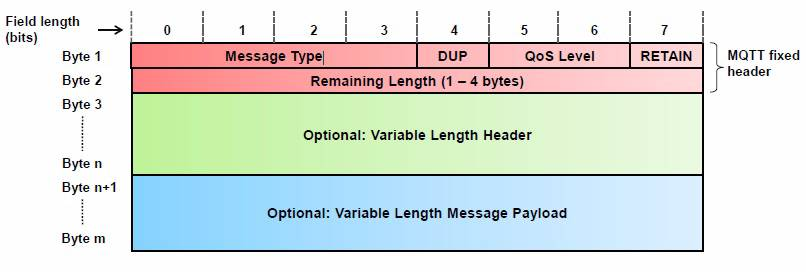
\includegraphics[width=\textwidth]{app/MQTT}
\end{figure}

\paragraph{Conclusioni} Sebbene l'implementazione MQTT non sia ancora stata rilasciata, i test evidenziati nella tabella \ref{fig:networkperformance} evidenziano il risparmio di risorse, sia in termini di consumo batteria, sia in termini di messaggi/ora gestibili (il quale è diretta conseguenza della bassa latenza).

\pagebreak

\begin{figure}[ht]
\centering
\caption{Confronto utilizzo risorse per i due protocolli HTTP e MQTT}
\label{fig:networkperformance}
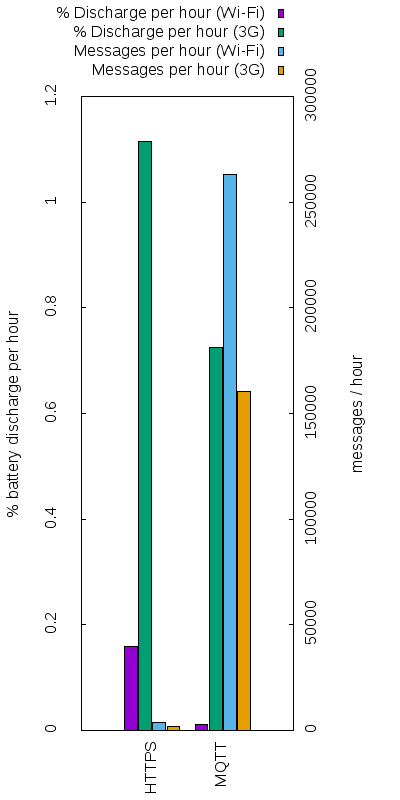
\includegraphics[scale=0.8]{database/networkperformance}
\end{figure}

\pagebreak

\section{Pushback}
\label{section:pushback}

\begin{wrapfigure}{r}{0.30\textwidth}

\includegraphics[width=0.30\textwidth]{app/hsit}
\end{wrapfigure}

Una sezione non critica della applicazione, ma molto importante dal punto di vista dell'analisi degli utenti e delle risposte al terremoto, è la parte denominata "\textit{Hai sentito il terremoto?}". Questa sezione della App fa parte dell'omonimo progetto dell'\textit{Istituto Nazionale di Geofisica e Vulcanologia}, che mira ad identificare e classificare la risposta emotiva e culturale degli utenti mediante un questionario sugli effetti del terremoto sul proprio stato d'animo e sugli oggetti intorno a se. Un classico esempio di utilizzo di questi dati è l'\textbf{analisi della differenza tra l'intensità/magnitudo del terremoto e la percezione di esso} che ha la popolazione residente: questo è dato, da INGV, come indice della cultura e della prevenzione contro i sismi.

\paragraph{La sezione del questionario} Il questionario, realizzato all'interno della applicazione, si compone di diverse domande a scelta singola o multipla, prima delle quali l'utente è invitato ad indicare la sua posizione nel momento in cui ha avvertito il terremoto. Alla fine della compilazione le risposte al questionario vengono inserite in un unico file JSON che viene inviato al server e condiviso con INGV (per generare la mappa \ref{fig:hsitmap}). Poiché lo sviluppo della sezione del questionario è avvenuta parallelamente alle ottimizzazioni, è stato possibile, fin dal principio, studiare un sistema efficace di invio affidabile e asincrono, in modo da garantire la consegna del questionario anche in condizioni di scarsa connettività, e soprattutto \textbf{in modo asincrono rispetto all'attività utente} (in altre parole l'utente, terminato il questionario, non deve attendere che l'invio sia completato con successo: sarà una attività eseguita in background). Questo ultimo punto è importante dal punto di vista della \textit{Human Interaction} poiché non c'è nessun motivo per far attendere l'utente per una operazione che non richiede il suo intervento.

\begin{figure}[ht]
\centering
\label{fig:survey1}
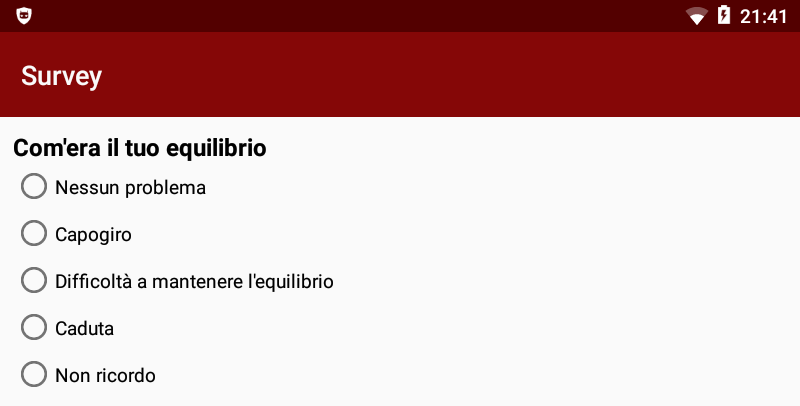
\includegraphics[width=0.6\textwidth]{app/survey2}
\caption{Schermata della applicazione di una delle domande del questionario}
\end{figure}

\paragraph{Il meccanismo di pushback} Per l'invio in background dei risultati del sondaggio, quindi, è stato ideato e realizzato un meccanismo, denominato \textit{di pushback}, che funziona in questo modo: è presente una coda di file\footnote{il meccanismo è stato ideato e sviluppato in modo generico, così ché in futuro si possa riutilizzare per altre tipologie di dati da sottomettere al server in asincrono ed in background} da inviare al server, ed un servizio in background di invio che viene svegliato per l'invio e/o ad intervalli non regolari. Il servizio, al risveglio, scorre la lista degli oggetti da inviare e tenta l'invio. Se fallisce (per problemi di rete o di altra natura), l'oggetto viene riaccodato per il prossimo ciclo.

\begin{figure}[ht]
\centering
\caption{Diagramma degli stati per il servizio di pushback}
\label{fig:scs_pb1}
\digraph[width=\textwidth]{PushBack1}{
rankdir=LR;
Start->DeQueueNext;
DeQueueNext->SendItem [label="ready"];
SendItem->DeQueueNext [label="sent"];
SendItem->QueueItem [label="failed"];
QueueItem->DeQueueNext;
DeQueueNext->End [label="end: empty"];
DeQueueNext->SetBackOff [label="end: not-empty"];
SetBackOff->End;
}
\end{figure}

E' importante notare che il servizio utilizza una particolare API di Android denominata \texttt{AlarmManager.setInexactRepeating}: l'obiettivo di questa API è di fornire uno strumento, agli sviluppatori, per poter schedulare delle operazioni ad intervalli \textit{non precisi}. \textbf{La non-precisione di questo metodo è il meccanismo chiave per il risparmio di risorse}: poiché non è necessario che l'operazione di pushback sia eseguita esattamente in un certo momento, è molto più corretto attendere un tempo variabile ed essere svegliati quando gli algoritmi di \textit{resources management} di Android decidono che è arrivato il momento opportuno (ad esempio quando il telefono è già in uso prima dell'intervallo, o se ci sono delle richieste di scheduling "esatte" inoltrate da altri servizi in un intorno del tempo specificato). Nel listato \ref{listing:pushback} è possibile vedere la chiamata nel codice.

Il servizio rimuove dalla coda, dopo 24 ore, gli elementi per cui l'invio è fallito, notificando eventualmente gli sviluppatori tramite un \textit{log collector} chiamato ACRA.

\begin{listing}[h]
\begin{minted}[mathescape,
               linenos,
               numbersep=5pt,
               gobble=0,
               frame=lines,
               framesep=2mm]{java}
serviceSingletonSemaphore.acquire();
PushbackDB db = new PushbackDB(this);
if (db.queueSize() > 0) {
	Intent receiverIntent = new Intent(this, WakeUpAlarmReceiver.class);
	backoffReceiverPendingIntent = PendingIntent.getBroadcast(
		this, 0, receiverIntent, 0);
	Calendar calendar = Calendar.getInstance();
	calendar.add(Calendar.MINUTE, 15);
	AlarmManager am = (AlarmManager) getSystemService(ALARM_SERVICE);
	am.setInexactRepeating(
			AlarmManager.RTC_WAKEUP,
			calendar.getTimeInMillis(),
			AlarmManager.INTERVAL_FIFTEEN_MINUTES,
			backoffReceiverPendingIntent
	);
}
serviceSingleton = false;
serviceSingletonSemaphore.release();
\end{minted}
\caption{Sezione di chiusura del servizio di pushback, dove viene impostato l'eventuale nuovo ciclo per gli elementi da inviare (se la coda li contiene)}
\label{listing:pushback}
\end{listing}

\begin{figure}[h]
\centering
\caption{Grafico dei report inviati dagli utenti che collaborano al progetto per il terremoto di Rieti del 24 agosto 2016 (ore 03:36)}
\label{fig:hsitmap}
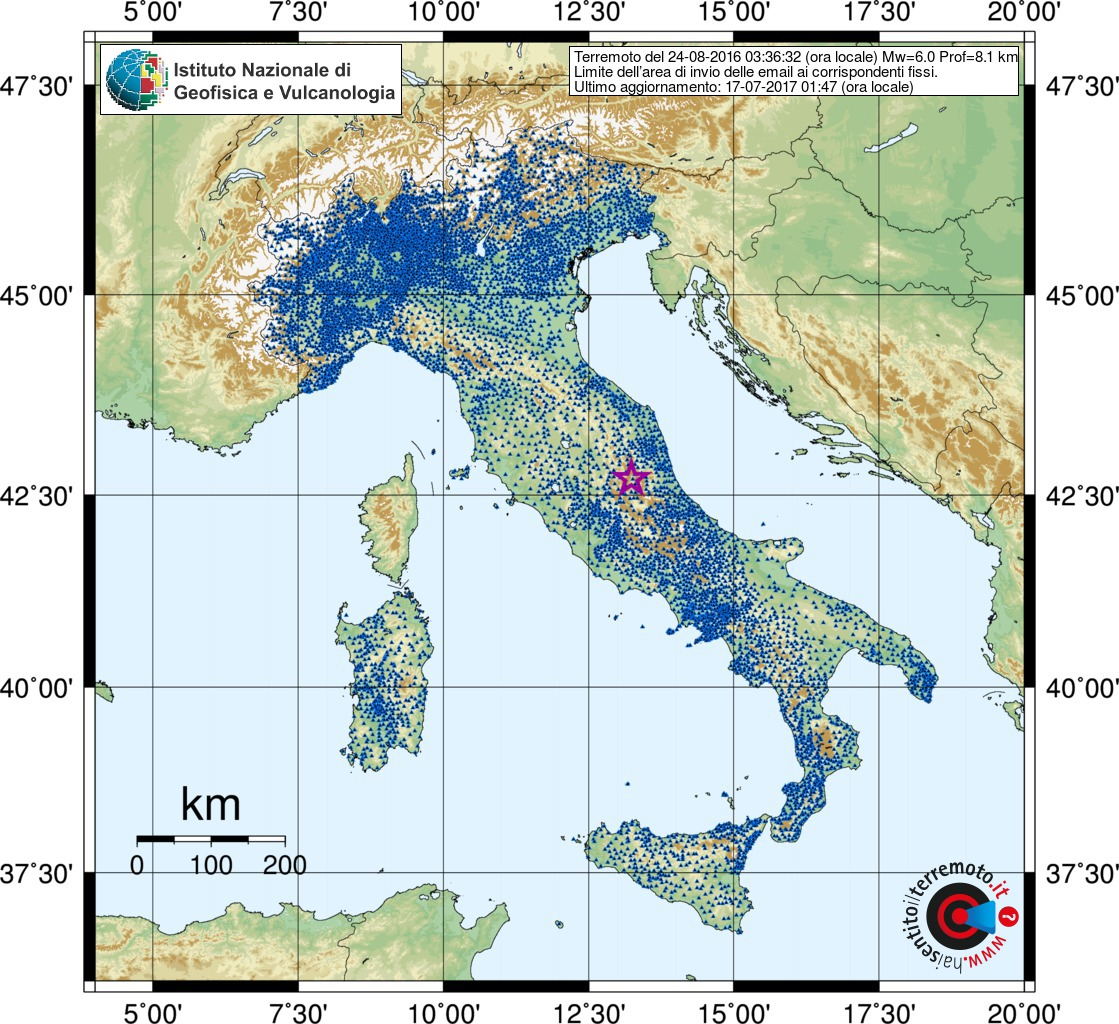
\includegraphics[width=\textwidth]{app/hsit_email}
\end{figure}

\chapter{Ottimizzazione dell'uso di memoria e CPU nel codice}

Infine, ma non meno importanti, altre due risorse da ottimizzare sono il tempo nel processore principale (CPU) e la memoria temporanea utilizzata (RAM). Anche in questo campo gli \textit{smartphones} hanno rappresentato un punto di svolta nella potenza di calcolo e nella capacità di memoria dei dispositivi cellulari. Eppure, la richiesta di nuove e più complesse funzionalità spinge sempre al limite la tecnologia, con chip che tentano di mantenere un basso consumo con potenze sempre più elevate. Anche in questo campo una buona progettazione della applicazione può portare benefici considerevoli.

\section{Transito dati tra front-end e servizio in background}

\paragraph{Activity lifecycle} Con \textit{Activity lifecycle} si intende il ciclo di vita di una schermata (che gli sviluppatori chiamano \textit{activity}) di una applicazione Android. Rispettare il ciclo di vita di una \textit{activity} è importante per rispettare le risorse che ci sono a bordo dello smartphone, specialmente, come in questo caso, quando la tipologia e la cardinalità dei dati potrebbe essere un problema \cite{activitylifecycle}.

\begin{figure}[h]
\centering
\caption{Ciclo di vita di una \textit{activity} Android}
\label{fig:activitylifecycle}
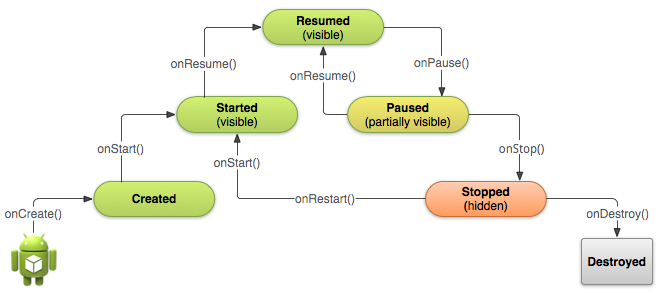
\includegraphics[width=\textwidth]{app/android_activity_lifecycle}
\end{figure}

In molte \textit{activity} è necessario interagire con il servizio in background di rilevamento, poiché ad esso sono lasciati diversi compiti tra cui, ad esempio, il compito di tracciare la posizione dell'utente: una tra le \textit{activity} che richiedono la posizione è la mappa dei terremoti, che necessita della posizione attuale per indicare la distanza dell'utente dall'epicentro.

Questo passaggio di dati avveniva, principalmente, attraverso l'interrogazione continua del servizio in background da parte della \textit{activity} corrente, per ogni activity. Poiché, in principio, erano stati considerati solo gli stati \textbf{Created} e \textbf{Destroyed} del ciclo di vita, fintanto che la \textit{activity} rimaneva in memoria, veniva utilizzato tempo di CPU e spazio RAM per trasportare i dati tra il servizio e la \textit{activity}, danneggando anche la \textit{user experience}.

\paragraph{Adeguamento del codice} E' stato quindi reingegnerizzato il codice delle \textit{activity} che lo richiedevano, adeguando le varie fasi al grafo degli stati in figura \ref{fig:activitylifecycle}:
\begin{itemize}
\item Ogni richiesta di un dato che può non cambiare per un tempo ragionevole (ad esempio, la provincia/regione dalla localizzazione) viene richiesto nel metodo \texttt{onStart()} e viene fatta una sola volta
\item Ogni richiesta di un dato che può variare poco nel tempo di utilizzo della App (ad esempio, lo stato del servizio in background) viene ricevuto, dalla \textit{activity}, per mezzo di un \texttt{BroadcastReceiver}, ovvero un sistema di sottoscrizione degli eventi
\item Ogni richiesta di un dato che può variare molto nel tempo di utilizzo della App (ad esempio il valore corrente di accelerazione letto dal servizio) viene interrogato mediante un servizio "di appoggio" della \textit{activity}, avviato nel metodo \texttt{onResume()} e fermato nel metodo \texttt{onPause()}, eventualmente distrutto nel metodo \texttt{onDestroy()}
\end{itemize}

Poiché lo stato di \textbf{Paused} viene invocato quando l'\textit{activity} non è più oggetto principale dell'attenzione dell'utente (ad esempio perché è subentrato un \textit{popup}), ogni qual volta si passa in questo stato viene risparmiata CPU e RAM rispetto all'attività precedente. Inoltre, se il dato è stato identificato come un dato che non cambia significativamente durante l'utilizzo della App, tale dato viene richiesto una sola volta o viene informata l'\textit{activity} tramite una segnalazione, e non un \textit{polling} come prima, e questo rappresenta di nuovo una ottimizzazione notevole.


\begin{listing}[h]
\begin{minted}[mathescape,
               linenos,
               numbersep=5pt,
               gobble=0,
               frame=lines,
               framesep=2mm]{java}
registerReceiver(new BroadcastReceiver() {
	@Override
	public void onReceive(Context context, Intent intent) {
		MySeismoActivity.this.runOnUiThread(new Runnable() {
			@Override
			public void run() {
				updateServiceStatusLed(...);
			}
		});
	}
}, new IntentFilter(Config.SERVICE_CHANGE_STATUS));
\end{minted}
\caption{Registrazione del \texttt{BroadcastReceiver} per il cambio di stato del servizio in background - porzione di codice dalla activity \texttt{MySeismoActivity} (activity principale)}
\end{listing}


\begin{listing}[h]
\begin{minted}[mathescape,
               linenos,
               numbersep=5pt,
               gobble=0,
               frame=lines,
               framesep=2mm]{java}
Location myLocation = null;
MySeismoService service = MySeismoService.getInstance();
if (MySeismoService.isServiceOn() && service != null) {
	myLocation = service.getLocation();
}
\end{minted}
\caption{Accesso, tramite \textit{singleton}, alla localizzazione acquisita dal servizio (se disponibile) - porzione di codice del metodo \texttt{onStart()} della \textit{activity} \texttt{Map2Activity} (mappa terremoti)}
\end{listing}

\section{Calcolo media e varianza online}
\label{section:onlinealg}

L'algoritmo di rilevamento specificato nella sezione~\ref{section:algoritmo} fa utilizzo della media e della varianza dei valori rilevati. Poiché la rilevazione viene fatta ogni $20ms$, ogni secondo di attività comporta la memorizzazione di 50 valori che, al netto dei puntatori e di altri riferimenti del runtime di Android, vuol dire un incremento minimo di 400 bytes/s, ovvero di 24KB al minuto. Inoltre, aggiornare la media ogni volta che si aggiunge un valore vuol dire eseguire una iterazione (tra tutti i valori memorizzati) per la somma della media, e una seconda iterazione per il calcolo dello scarto quadratico medio, con un tempo complessivo di $\Theta(nm)$ per ogni valore rilevato (50 volte al secondo).

\paragraph{Algoritmi \textit{online}} Per ridurre il consumo di memoria ed l'utilizzo della CPU per il ricalcolo della media ad ogni valore, si è utilizzato un algoritmo definito \textit{online}\footnote{Un algoritmo viene definito \textit{online} se è in grado di processare un oggetto di input per volta (mantenendo l'invariante che il risultato rappresenta il valore atteso), potenzialmente per un numero infinito di oggetti. \cite{onlinealg}}, che effettua il calcolo della media e dello scarto quadratico medio al momento, e non richiede la memorizzazione di tutti i valori. Questo è possibile grazie alla definizione e all'utilizzo delle relazioni di ricorrenza per la media (formula~\ref{eq:avgrec}) e per lo scarto quadratico medio (formula~\ref{eq:sqmrec}) \cite{onlineavg}.

\begin{equation}
\Delta = Acceleration - M_{i-1}
\end{equation}
\begin{equation}
\label{eq:avgrec}
M_i = M_{i-1} + {\Delta \over |detections|}
\end{equation}
\begin{equation}
\label{eq:sqmrec}
\sigma_i = \sigma_{i-1} + \Delta * (Acceleration - M_i)
\end{equation}

dove: \begin{itemize}
\item $Acceleration \in Z^+$ rappresenta il valore di accelerazione attuale
\item $|detections| \in N^+, |detections| > 0$ rappresenta il numero di rilevazioni fatte fin'ora
\item $\Delta \in Z^+$ rappresenta la differenza tra l'accelerazione e la media attuale
\item $M_i \in Z^+$ è la media dei valori delle rilevazioni
\item $\sigma_i \in Z^+$ è lo scarto quadratico medio
\end{itemize}

L'occupazione di memoria, grazie all'utilizzo di questo algoritmo, è costante nel tempo. Inoltre, la complessità di questo algoritmo è $\Theta(1)$.

\chapter{Ottimizzazione in fase di sviluppo}

Una buona ottimizzazione è sicuramente salutare per un software, ma non dobbiamo dimenticarci che \textit{l'ottimizzazione non è un prodotto, ma un processo}. Dobbiamo quindi assicurarci che il nostro lavoro non vada perduto nel quotidiano, cercando metodi che ci aiutano ad applicare correttamente le \textit{best practices} e allo stesso tempo notificarci dei problemi, possibilmente nel modo più rapido e automatico possibile (così da concentrarci sui veri problemi).

\section{Android Annotations}
\label{section:aa}

\begin{flushright}
``\textit{If debugging is the process of removing software bugs, then programming must be the process of putting them in.}" \\ Edsger Dijkstra
\end{flushright}

L'apertura di finestre, il controllo di alcuni valori, la gestione dei processi in background richiedono molto codice, spesso usato a ripetizione con poche variazioni. A volte, come è capitato in questa applicazione, alcuni processi non sono ottimali. \textbf{Una regola d'oro quindi è: meno codice c'è, meno codice è da mantenere e ottimizzare}. Vediamo come possiamo ottimizzare la nostra app scrivendo meno codice.


\begin{wrapfigure}{r}{0.10\textwidth}

\includegraphics[width=0.10\textwidth]{dev/aa}
\end{wrapfigure}

\paragraph{Android Annotations} Una libreria di terze parti che realizza una vera e propria rivoluzione nell'eliminazione del codice ridondante si chiama \textbf{Android Annotations}. Inizialmente, come suggerisce il nome, era una collezione di annotazioni di Java utili per Android, ma si è evoluta fino ad inglobare ed automatizzare numerosi e macchinosi "\textit{task}" che gli sviluppatori si trovano a fare.

\medskip

Le \textbf{annotazioni} in Java sono un tipo di \textit{metadato} che può essere aggiunto ad ogni attributo, classe, metodo o attributo di un metodo. Questo metadato è trasportato nel \textit{bytecode} Java, in modo da essere accessibile tramite \textit{reflection}\footnote{\textit{Reflection} è un modo di accesso agli attributi e metodi di una classe in modo dinamico, ovvero senza che si conosca a tempo di compilazione la struttura. E' utilizzata per costruire dei sistemi di caricamento dinamico delle librerie, ad esempio.}. Può essere utile sia in fase di compilazione o analisi statica (ad esempio, se aggiungo l'annotazione \texttt{@NonNull} un sistema di verifica può analizzare staticamente il codice e controllare se ci sono casi in cui ritorna \texttt{NULL}, ed in quel caso emettere un errore), oppure è utile in \textit{runtime} (ad esempio, si può scorrere tramite reflection gli attributi di una classe e lavorare solo su quelli annotati, senza sapere staticamente quali sono in fase di compilazione).

\medskip

In Android, ad esempio, quando è necessario leggere le informazioni passate dalla \textit{activity} chiamante, in genere il codice da scrivere è:

\begin{listing}[H]
\begin{minted}[mathescape,
               linenos,
               numbersep=5pt,
               gobble=0,
               frame=lines,
               framesep=2mm]{java}
               
public class SurveyActivity extends AppCompatActivity {
	private String param1;
	private String param2;

	@Override
	protected void onCreate(Bundle savedInstanceState) {
		super.onCreate(savedInstanceState);
		setContentView(R.layout.activity_survey);
		
		Intent in = getIntent();
		if (in == null) {
			// Gestione dell'errore
			this.finish();
		}
		param1 = in.getStringExtra("param1");
		param2 = in.getStringExtra("param2");
	}
	// Altro codice della activity
}
\end{minted}
\end{listing}

Mentre lo stesso effetto si ottiene con:

\begin{listing}[H]
\begin{minted}[mathescape,
               linenos,
               numbersep=5pt,
               gobble=0,
               frame=lines,
               framesep=2mm]{java}
@EActivity(R.layout.activity_survey)
public class SurveyActivity extends AppCompatActivity {
	@Extra String param1;
	@Extra String param2;
	// Altro codice della activity
}
\end{minted}
\end{listing}

Chiaramente usare \textbf{Android Annotations} ha molti vantaggi. Si è stimato che il codice diminuisce in media di circa il 30\%\footnote{secondo gli autori della libreria}. Inoltre, alcuni passaggi sono molto più intuitivi (ad esempio, la presenza della annotazione \texttt{@Extra} di fianco alla dichiarazione di \texttt{param1} nel codice indica subito che si tratta di un parametro proveniente dall'esterno della \textit{activity}). L'adozione di questa libreria è stata fatta in modo graduale, poiché non è necessario utilizzarla in modo esclusivo rispetto alle tecniche standard di Android.

\clearpage

\section{LeakCanary}

\begin{flushright}
``\textit{A small leak will sink a great ship.}" \\ Benjamin Franklin
\end{flushright}

\medskip

Un \textbf{memory leak} è una condizione nella quale un software non rilascia un'area di memoria (che sia essa una variabile, un array, etc) ma perde la possibilità di utilizzarla (per effettiva perdita del \textit{puntatore}, ad esempio) e/o dimentica di liberarla. Sebbene nell'immediato non sia un grosso problema (a meno di grandi allocazioni), per qualcosa che rimane in esecuzione per molto tempo (nel nostro caso ad esempio, il servizio di rilevamento di scosse) rappresenta un grave problema, specialmente se tale \textit{leak} avviene dentro codice che viene iterato spesso (poiché l'effetto si somma).

\paragraph{LeakCanary} Una libreria di terze parti, chiamata \textbf{LeakCanary}\footnote{\textit{Canary} è la parola inglese per specificare "canarino"; l'utilizzo di questo animale come esempio è frequente nell'informatica, specialmente nella sicurezza. E' preso in prestito dalla storia dei minatori di carbone, i quali portavano un canarino nelle grotte: se il canarino, più sensibile alla mancanza di ossigeno, moriva, esso era il segnale di allarme per abbandonare il posto prima di morire asfissiati} si preoccupa di controllare, durante la fase di test nello sviluppo ed in modo del tutto trasparente dal punto di vista del codice, ogni allocazione e deallocazione in memoria effettuata dalla nostra applicazione o dalle librerie utilizzate. Qualora si venga a creare un \textit{memory leak}, l'applicazione \textbf{raccoglie i dati sulle cause e le segnala allo sviluppatore immediatamente}. Questo permette di correggere la maggior parte dei \textit{memory leaks}.


\begin{figure}[ht]
\centering
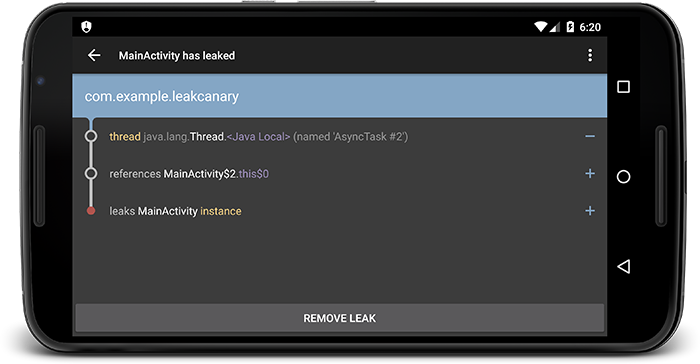
\includegraphics[width=0.8\textwidth]{dev/leakcanary}
\caption{Lo stacktrace di una chiamata di esempio (che finisce con un \textit{leak}), mostrata da LeakCanary sullo smartphone di sviluppo}
\end{figure}

\clearpage

\section{Application Crash Reports for Android}

\begin{flushright}
``\textit{It's not a bug – it's an undocumented feature.}" \\ Anonymous
\end{flushright}

Ogni software sviluppato non è esente da errori di programmazione. Per quanto un software possa essere controllato, ricontrollato, sottoposto a stress e verifiche di funzionamento, ci sarà sempre la possibilità che un errore si annidi all'interno della più complessa componente del sistema. E ovviamente spesso questo \textit{bug}\footnote{Si utilizza la parola inglese \textit{bug} per indicare gli errori di sistema, in genere di programmazione, da quando in un lontano passato un insetto (da qui la parola \textit{bug}), entrando dentro gli ingranaggi di una delle prime macchine per il calcolo automatico, bloccò il suo funzionamento fino alla completa ispezione.} si presenta nell'ambiente di "produzione", ovvero nel telefono dell'utente. E' quindi utile tener traccia di questi problemi, perché non sempre questi causano il blocco completo dell'applicazione: potrebbero comportare utilizzi eccessivi della rete o in generale delle risorse a bordo del telefono.

\begin{wrapfigure}{r}{0.10\textwidth}

\includegraphics[width=0.10\textwidth]{dev/ACRA}
\end{wrapfigure}

\paragraph{ACRA} Un componente che è stato aggiunto alla nostra applicazione si chiama \textbf{Application Crash Reports for Android} (ACRA). Lo scopo di questo componente è quello di individuare i problemi (i \textit{crash} dell'applicazione), oppure di raccogliere le segnalazioni fatte in modo volontario, nel codice sorgente, da parte del programmatore, ed inviarle ad un sistema centrale per l'analisi e la gestione. Le informazioni inviate contengono i dettagli del problema, oltre che ai dettagli della piattaforma su cui l'applicazione sta girando (in modo che gli sviluppatori possano riprodurre l'ambiente, e, si spera, riprodurre il \textit{bug}).

ACRA si compone di un backend, chiamato \textit{ACRAlyzer}, il quale funge da collettore per i report inviati dalla componente ACRA che gira nel telefono Android. Tuttavia abbiamo dovuto abbandonare tale backend per problemi di performance: esso faceva pesante uso di CouchDB, il quale, per il nostro tipo di interrogazione, era notevolmente inefficiente. Ho quindi dovuto scrivere un middleware in Python, il quale adesso è un progetto \textit{open-source} su GitHub\footnote{\url{https://github.com/Enrico204/acraflask}} chiamato \textbf{ACRAFlask}, per poter gestire i dati in ingresso, utilizzando un database NoSQL chiamato \textbf{OrientDB}, il quale permette una buona versatilità e riesce a gestire correttamente il carico di lavoro della app \textbf{SeismoCloud}.

Grazie ad ACRAFlask il \textit{team} di sviluppo è in grado di identificare per tempo non solo i \textit{crash} applicativi, ma di mettere in relazione tali \textit{crash} e le \textit{performance} dell'applicazione con le caratteristiche fisiche del telefono.

\begin{figure}[ht]
\centering
\caption{Flusso di informazioni per i log dei crash}
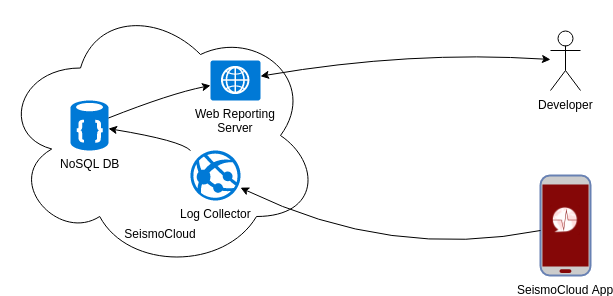
\includegraphics[width=0.6\textwidth]{dev/acracollector}
\end{figure}

\begin{figure}[ht]
\centering
\caption{ACRAFlask, il progetto \textit{collector} per i report di ACRA}
\label{fig:acraflask}
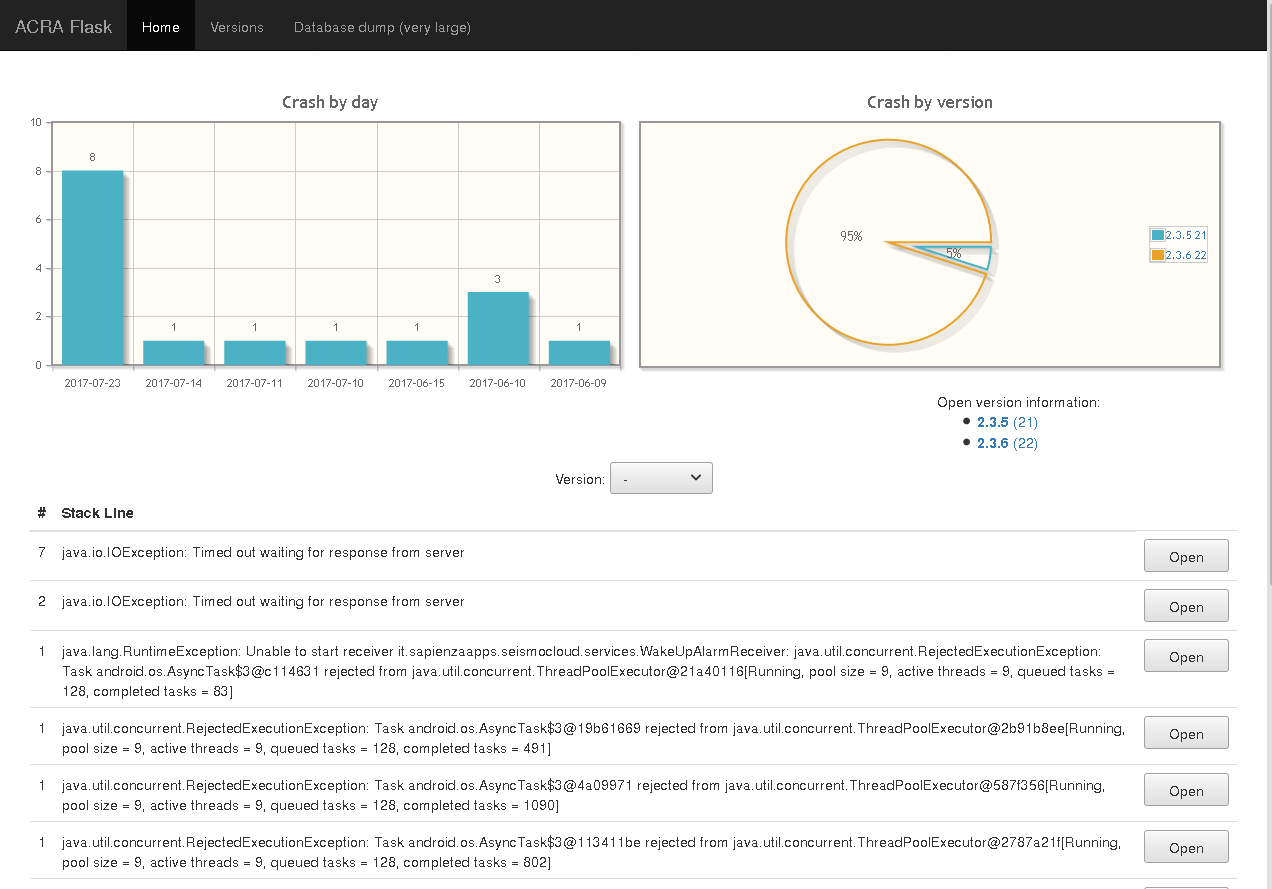
\includegraphics[width=\textwidth]{dev/acraflask}
\end{figure}

\clearpage

\section{Continuous Integration}
\label{section:ci}

Poiché l'ottimizzazione non è un prodotto ma un processo, si è deciso di creare una \textit{pipeline}, ovvero una serie di processi, per iniziare con un processo di \textit{continuous integration}. La \textit{pipeline} di \textit{continuous integration} che abbiamo scelto di implementare prevede alcuni step: la creazione di un \textit{repository centrale} di codice gestito tramite un sistema di controllo versione (VCS); la generazione di build automatiche; l'analisi statica del codice e l'implementazione di test strumentali.

\begin{figure}[ht]
\centering
\caption{I passi del nostro sistema di Continuous Integration}
\digraph[width=\textwidth]{CIStateMachine}{
rankdir=LR;
{
Build->Analyze [label="Build ok"];
Build->Report [label="Build error"];
Analyze->Test [label="Quality Gate ok"];
Analyze->Report [label="Quality Gate error"];
Test->Done [label="Test ok"];
Test->Report [label="Test error"];
Report->Done;
}
{
rankdir=TB;
rank=min;
Get->Build;
}
}
\end{figure}

Il sistema di Continuous Integration che abbiamo installato si compone di un "direttore d'orchestra" chiamato \textbf{Jenkins}, il quale si occupa di eseguire, in automatico ad un orario prestabilito, i passi di:
\begin{itemize}
\item Recupero dell'ultima versione del codice sorgente dal VCS tramite \texttt{git}
\item Compilazione, mediante l'\textbf{Android SDK}, del codice: questo assicura che il codice presente sia effettivamente compilabile e che ci siano tutti i file
\item Analisi del codice statica: tramite uno strumento chiamato \textbf{SonarQube} (ed altri tool a supporto) viene effettuata l'analisi statica del codice sorgente Java/Android: vengono effettuati diversi controlli per l'individuazione di bug e di errori di leaks nel codice, inoltre vengono applicate delle regole stringenti sul \textit{code-styling}, in modo da minimizzare la presenza di errori
\item Test strumentali: viene simulata l'interazione con l'utente (mediante finte pressioni e inserimenti di testo) nel simulatore di Android, allo scopo di far uscire bug e leaks
\end{itemize}

Quando un passo fallisce, vengono notificati gli sviluppatori. Inoltre si mantiene lo storico di queste analisi per poter effettuare dei miglioramenti futuri al processo di sviluppo.

\begin{figure}[ht]
\centering
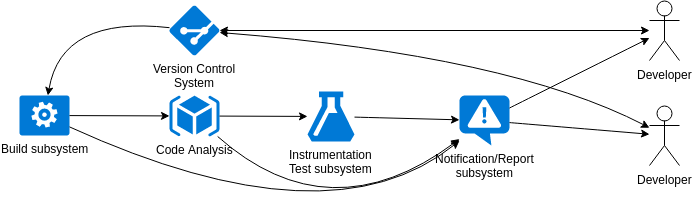
\includegraphics[width=0.9\textwidth]{dev/ci}
\caption{Visione d'insieme del sistema di \textit{continuous integration}}
\end{figure}

\chapter{Conclusioni}

\section{Risultati ottenuti}

Abbiamo visto come poter modificare l'applicazione allo scopo di ottimizzare l'utilizzo delle risorse, per primo il \textbf{consumo della batteria}: considerando i contesti di attivazione per il risparmio energetico (sezione~\ref{section:contesti}), riducendo l'impatto della comunicazione con il frontend (sezione~\ref{section:frontend}), e, passando per una buona gestione dei sensori (sezione~\ref{section:sensori}), per arrivare alla definizione ed uso di una curva di scarica (sezione~\ref{section:curvascarica}).

\medskip

Un secondo passaggio ci ha permesso di \textbf{ottimizzare la comunicazione con il server}, grazie all'implementazione di MQTT (sezione~\ref{section:mqtt}) e di un sistema chiamato \textit{pushback} (sezione~\ref{section:pushback}).

\medskip

Un minore, ma comunque importante contributo lo ha dato l'\textbf{ottimizzazione dell'uso di memoria e di CPU}, per i quali sono stati affrontati i problemi del transito dei dati tra front-end e servizio (sezione~\ref{section:frontend}) e l'algoritmo di calcolo della soglia per le parti di media e varianza (sezione~\ref{section:onlinealg})

\medskip

Infine, sono state introdotte nuove librerie in grado di generare in modo ottimale il codice ridondante (sezione~\ref{section:aa}), ed è stato introdotto un sistema di \textit{pipeline} per monitorare costantemente l'uso delle risorse all'interno delle build nel processo di sviluppo (sezione~\ref{section:ci}).

\vspace*{1cm}

\textbf{L'applicazione}, con questo livello di ottimizzazione, \textbf{è in grado di consumare le risorse in modo molto più efficace di prima}, migliorando l'usabilità dello smartphone e garantendosi una migliore coesistenza all'interno dello stesso.

\clearpage

\section{Sviluppi futuri}

Durante lo sviluppo di questa tesi (e delle soluzioni esposte) sono emersi diversi punti che possono portare ad ottimizzazioni ulteriori nel funzionamento della applicazione.

\subsection{Sistema di spegnimento controllato}

Un ulteriore passo, esplorato in fase di progettazione ma mai realizzato né testato, è lo spegnimento controllato dal server in base alla quantità di sismometri presenti in una determinata zona: poiché l'algoritmo si basa sulla quantità di sismometri per l'affidabilità, quando il numero di dispositivi è elevato e si è raggiunto un livello accettabile di affidabilità non è più necessario che altri (diversi) dispositivi, in una certa zona, siano attivi: \textbf{il server potrà quindi decidere di spegnere a turno i servizi di rilevamento per conservare la batteria}.

\subsection{Studio sull'utilizzo di sensori dedicati}

Alcuni telefoni hanno a bordo diverse tipologie di sensori (virtuali e non) in grado di fornire le stesse (o maggiori) informazioni che attualmente vengono lette per ottenere lo stesso scopo. L'utilizzo di questi sensori potrebbe portare un notevole risparmio energetico. Un esempio è il sensore (attualmente trovato solo sui dispositivi Samsung) chiamato "Significant Motion Sensor": qualora questo sensore abbia la capacità di individuare movimenti significativi per le caratteristiche richieste dalla app \textbf{SeismoCloud}, potrebbe essere implementato un sistema di stand-by del servizio con consumi molto più ridotti rispetto a quelli attuali.

\subsection{Scrittura del codice nativo (C/C++) per le componenti critiche}

Nonostante la \textit{virtual machine} Android sia notevolmente migliorata nel tempo, per alcune particolari funzioni può essere interessante esplorare la scrittura del codice nativo in \texttt{C/C++}, in particolare della parte di rilevazione delle scosse sismiche. Tale componente, poiché compilata in codice nativo, potrebbe risultare più veloce e più performante (e quindi, più \textit{green} dal punto di vista dei consumi).

\subsection{Esplorare ed implementare altre tecniche}

Durante la scrittura di questa tesi ed i test finali sono state individuate diverse tecniche, ulteriori o alternative, di ottimizzazione \cite{altrepub} per il monitoraggio continuo della posizione geografica di un dispositivo \textit{mobile}. Se compatibili con la App e con le implementazioni già in essere, è interessante capire se e quanto riescono ad ottimizzare ulteriormente il risparmio energetico.

\refstepcounter{chapter}
\chapter*{Ringraziamenti}

Sono tante le persone che ho incontrato nel mio percorso universitario, sia dentro che fuori le mura de \textit{La Sapienza}, e che hanno contribuito, direttamente o indirettamente, allo sviluppo di questa tesi.

\medskip

Vorrei iniziare ringraziando, prima di tutto, il relatore di questa tesi, il \textbf{Prof.~Emanuele Panizzi}, poiché è suo il merito di aver iniziato un progetto così innovativo, e di avermi coinvolto. Senza di lui, questo progetto e questa tesi non esisterebbero. Un contributo importante, per questo progetto, è da riconoscere anche al \textbf{Dr.~Salvatore Barba} e al \textbf{Dr.~Valerio De Rubeis}, entrambi ricercatori dell'Istituto Nazionale di Geofisica e Vulcanologia, per la componente sismologica.

\medskip

Fondamentale è stato il contributo di tanti ragazzi, ``colleghi", che ho incontrato nel tempo: \textit{Mario}, \textit{Marco}, \textit{Lorenzo} e \textit{Giulio } del primo gruppo di \textit{SeismoCloud}. \textit{Alessio}, per i tanti consigli che mi ha regalato. Ed in special modo \textit{Beatrice}, a cui devo molto.

\medskip

Un ringraziamento speciale, per avermi sempre sostenuto, va alla mia amica \textit{Raffaella}. Senza di lei non sarei arrivato dove sono ora.

\medskip

Non posso non ringraziare la mia famiglia, che mi è stata accanto in questi anni. Infine, ma non meno importanti, ringrazio gli amici, i conoscenti, il mio amico ed ex-collega \textit{Sandro} e tante altre persone che hanno contribuito a questo percorso.

\cleardoublepage

\refstepcounter{chapter}

\begin{thebibliography}{9}

\bibitem{introdseismo}
	\textbf{An Introduction to Seismology, Earthquakes, and Earth Structure}. \\
	Seth Stein; Michael Wysession (2009). John Wiley \& Sons. ISBN 978-1444311310

\bibitem{eqpred}
	\textbf{Short-term earthquake prediction: Current status of seismo-electromagnetics}. \\
	Seiya Uyeda; Toshiyasu Nagao; Masashi Kamogawa (2009-05-29), Tectonophysics, 470 (3–4): 205-213

\bibitem{alessamato}
	\textbf{Sotto i nostri piedi}. \\
	Alessandro Amato (2016). Codice edizioni, Torino. ISBN 978-8875785727

\bibitem{jma}
	\textbf{JMA, Japan Meteorological Agency}. \\
	\url{http://www.jma.go.jp/jma/en/Publications/publications.html}

\bibitem{eewapp}
	\textbf{Rapid Detection of Rare Geospatial Events: Earthquake Warning Applications}. \\
	Michael Olson; Annie Liu; Matthew Faulkner; Chandy K. Mani; DEBS '11, pp. 89-100, July 2011, ISBN 978-1-4503-0423-8

\bibitem{finazzi}
	\textbf{A statistical approach to crowdsourced smartphone-based earthquake early warning systems} \\
	Francesco Finazzi, Alessandro Fassò; Stochastic Environmental Research and Risk Assessment.  doi:10.1007/s00477-016-1240-8

\bibitem{gyroman}
	\textbf{L3G4200D Gyroscope datasheet} \\
	\url{https://cdn.sparkfun.com/datasheets/Sensors/Gyros/3-Axis/CD00265057.pdf}

\bibitem{accelman}
	\textbf{ADXL345 Accelerometer datasheet} \\
	\url{http://www.analog.com/media/en/technical-documentation/data-sheets/ADXL345.pdf}

\bibitem{ivlatb}
	\textbf{ISIDe (\textit{Italian Seismological Instrumental and parametric Data-base})} \\
	\textit{IV.LATB} sensor technical specifications, \url{http://iside.rm.ingv.it/iside/standard/info_stazione.jsp?page=sta&sta=1651&lang=it}

\bibitem{doze}
	\textbf{Understading Doze}. \\
	Android Developers documentation, \url{https://developer.android.com/training/monitoring-device-state/doze-standby.html}

\bibitem{http}
	\textbf{RFC 7230, Hypertext Transfer Protocol (HTTP/1.1)}: Message Syntax and Routing

\bibitem{mqtt}
	\textbf{MQTT Version 3.1.1 protocol specification}. \\
	\url{http://docs.oasis-open.org/mqtt/mqtt/v3.1.1/os/mqtt-v3.1.1-os.pdf}

\bibitem{activitylifecycle}
	\textbf{Activity-lifecycle concepts}. \\
	Android Developers documentation, \url{https://developer.android.com/guide/components/activities/activity-lifecycle.html}

\bibitem{onlinealg}
	\textbf{On-Line Algorithms versus Off-Line Algorithms: How Much is it Worth to Know the Future?} \\
	Richard M. Karp, July 1992, ICSI TR-92-044

\bibitem{onlineavg}
	\textbf{Algorithms for calculating variance}. \\
	Wikipedia, \url{https://en.wikipedia.org/wiki/Algorithms_for_calculating_variance}

\bibitem{altrepub}
	\textbf{Energy-Accuracy Trade-off for Continuous Mobile Device Location}. \\
	Kaisen Lin, Aman Kansal, Dimitrios Lymberopoulos, Feng Zhao; MobiSys '10 Proceedings of the 8th international conference on Mobile systems, applications, and services; ISBN: 978-1-60558-985-5

\end{thebibliography}

\begin{appendices}
\chapter{Diagramma di flusso completo del servizio}
\begin{figure}[ht]
\centering
\label{fig:serviceflowdiagram}
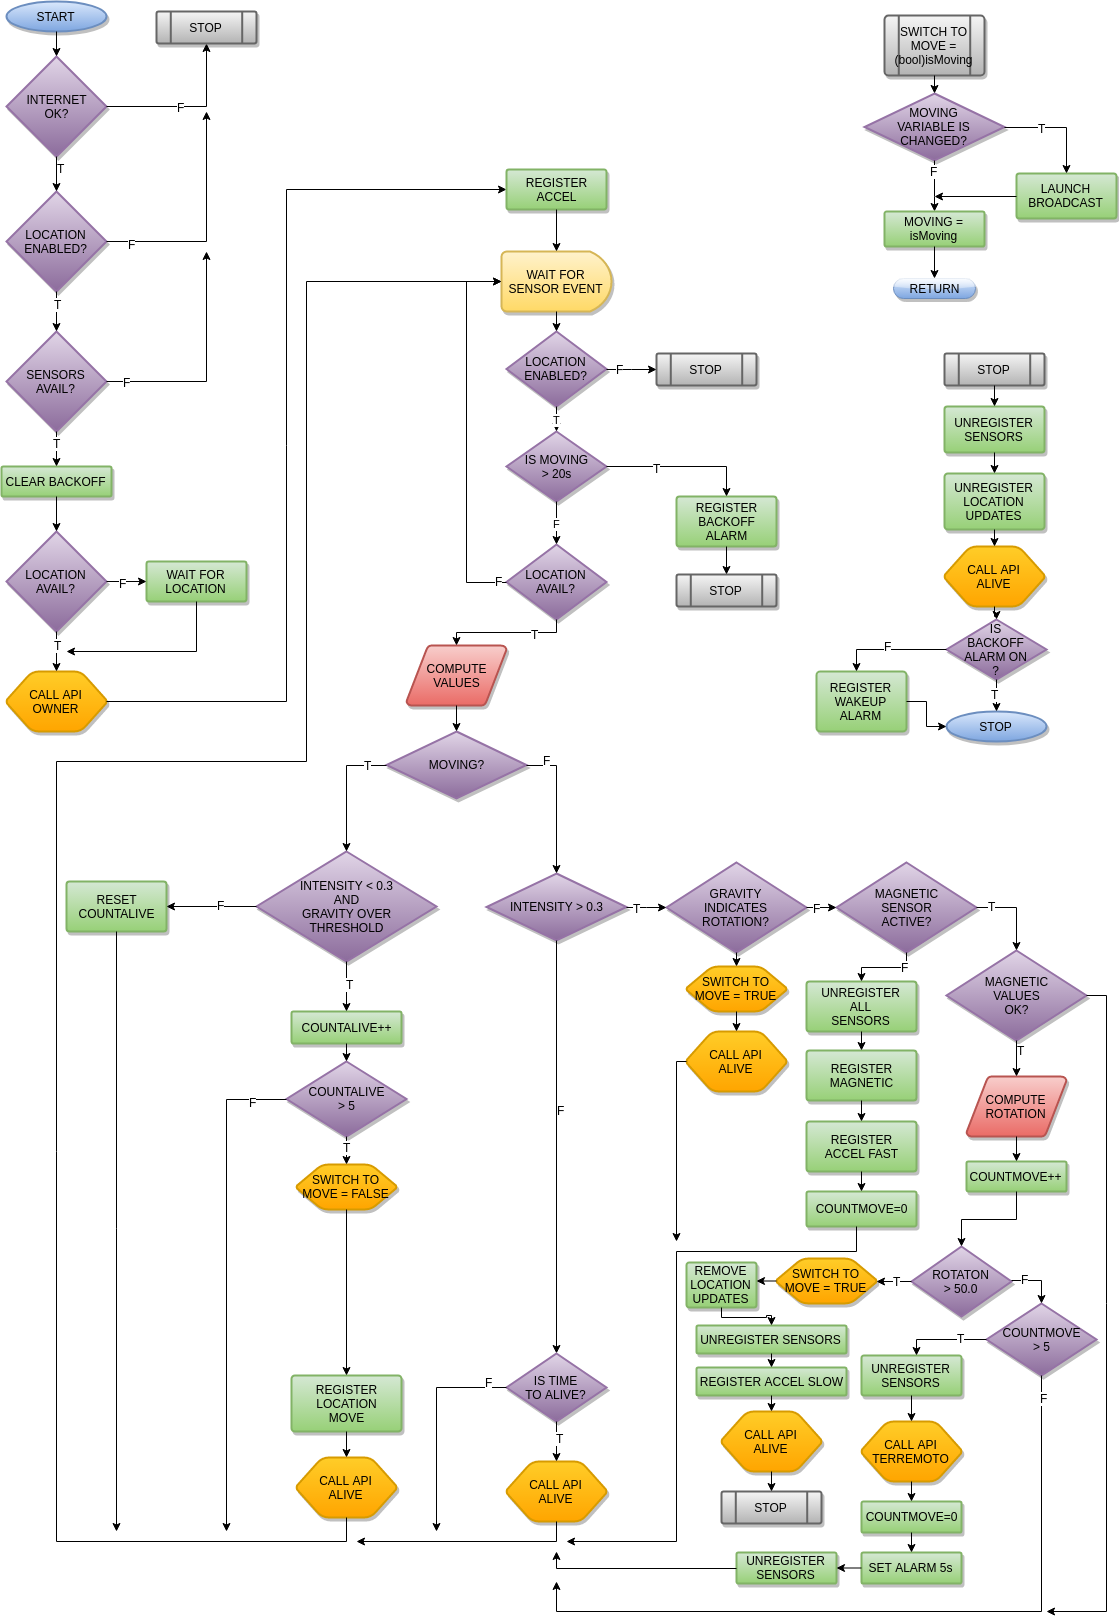
\includegraphics[width=0.8\textwidth]{SeismoCloud_flowdiag}
\end{figure}
\end{appendices}

\end{document}
